\documentclass{article}
\usepackage[a6paper, total={105mm, 148mm},margin=30pt]{geometry}
\usepackage[utf8]{inputenc}
\usepackage{graphicx}
\usepackage{parselines}
\usepackage[none]{hyphenat}
\usepackage{gensymb} %för att kunna använda symboler som grader
\usepackage{multicol} %För att få dubbla kolumner hos EBBE
\usepackage{ragged2e} %För att justifya text (dvs högercentrering och liknande
\usepackage{pdfpages} %för att inkludera pdf-bilder
\usepackage[export]{adjustbox} %Border på bilder
\usepackage{imakeidx}% registret
%\usepackage{tocloft} %för att ändra storlek på innehållsförteckningen
\usepackage[titles]{tocloft}
\usepackage{textcomp} % ~
\usepackage{pgffor, ifthen} %bortsupen
\usepackage{fancyhdr}


\fancypagestyle{main}{ 
\fancyhf{} % clear all header fields
%\fancyhead[LE]{\footnotesize\scshape\leftmark}
\fancyhead[RO]{\hfill \footnotesize\scshape\leftmark \hfill}
\fancyfoot[LE,RO]{\hfill \thepage \hfill}
\renewcommand{\headrulewidth}{0 pt}
\renewcommand{\footrulewidth}{0 pt}
}

\pagestyle{main}



\newcommand{\bortsupen}[3][\empty]{%
    \noindent \vspace{0pt}\\
    \foreach \n in {1,...,#2}{%
        \ifthenelse{\equal{#1}{\empty}}
            {\rule{#3}{0.5pt}\\}
            {\rule{#3}{0.5pt}\vspace{#1}\\}
        }
}

\newcommand{\fillInPages}[1]{
\newcount\ipp
\ipp=0
\newcount\numberOfPages
\numberOfPages=#1 
\loop
\newpage
\mbox{}
\advance\ipp by1
\ifnum\ipp<\numberOfPages\repeat
}





\makeindex[name=alfa, columns=1, title=Alfabetiskt Register, intoc, options = {-s styleAlfa.ist}]% också register - alfabetiskt
\makeindex[name=anfa, columns=1, title=Analfabetiskt Register, intoc, options = {-s styleAlfa.ist}]% också register - "analfabetiskt" eller början av sången



\title{\fontsize{20}{20} \selectfont D-sektionens sångbok \vspace{-40pt}}


\author{}
\date{}
\topmargin=-65pt
\headsep=10pt
\textheight=360pt
\footskip=15pt

\renewcommand*\contentsname{INNEHÅLL}
\setcounter{tocdepth}{1}
\setcounter{secnumdepth}{0}
\renewcommand\cftsecfont{\normalsize}                    %Font på table of content
\renewcommand\cftsecpagefont{\normalsize}                %Font på table of content
\setlength{\cftbeforesecskip}{3pt}                       %vspace på table of content


\tolerance=700

%\fancyfoot[R]{\thepage\ifodd\value{page}\hfill\value{page}\else\hfill\fi} %FUCK DETTA JAG GER UPP





\begin{document}


\thispagestyle{empty}
\maketitle
\thispagestyle{empty} %tar bort sidnumrering

\begin{center}
Trettionio råsa år - och ett brunt... 
\end{center}
\vspace{1mm} %den flyttar upp väldigt mycket mer om jag inte har med detta



\begin{center}
   %
\includepdf[width=0.1\textwidth]{D-symbol.pdf}
   
\includegraphics[width=0.6\textwidth]{res/D-symbol.pdf}
\end{center}



%\fancyhf{} % sets both header and footer to nothing
%\renewcommand{\headrulewidth}{0pt}
\newpage
Tillhör:
\newpage
\thispagestyle{plain}
\tableofcontents
\newpage
\thispagestyle{empty}
\section{Gasquelogi}
\subsection{Klädkod}
\subsubsection{Högtidsdräkt/högtidsklädsel}
För honom är frack lämplig. En fin golvlång klänning
gäller för henne - ett bra material och ett tjusigt snitt ska
det vara på den. Vill man bära handskar till klänningen
går det bra, men glöm inte att ta av dem när du äter.
Både han och hon kan istället bära hembygdsdräkt eller
militär högtidsdräkt.
\subsubsection{Smoking}
Då klädkoden är smoking, innebär det för honom en svart
eller mörkblå sådan. Förutom smokingjacka och byxa
ingår en särskild skjorta samt svart fluga. Hon har en lång
klänning, men den behöver inte vara lika elegant som vid
högtidsklädsel. Den får gärna vara festlig och glittrig.
Även kortare klänning - dock inte kortkort - går bra.
\subsubsection{Mörk kostym}
Han bär en mörkblå, mörkgrå eller svart kostym. Till det
har han en vit skjorta och sidenslips eller fluga i valfri färg
- gärna mönstrad! Hon har en klänning av siden, sammet
eller annat finare material. En elegant byxdress eller
halvlång kjol med jacka kan också bäras.

\subsubsection{Kavaj}
Tolkningen av kavaj kan variera. Om det är lite mer
högtidligt kan han bära mörk kostym. Är det mindre
formellt passar t.ex. en elegant blazer och udda byxa,
eller en ljusare kostym bra. Hon kan ha klänning, kjol eller
dress av varierande finhetsgrad beroende på
tillställningen. En hellång kjol eller klänning används inte.

\subsubsection{Vårdad klädsel}
Detta är egentligen ingen allmänt vedertagen klädkod,
men på LTH används den ibland. Det innebär i vilket fall
att man ska vara hel och ren, vilket många tolkar som
skjorta med snyggare byxor till. Undvik mjukisbyxor,
stövlar och saker som är jordiga.

\subsubsection{Ouveralle}
Som det låter. Bra att ha när man vill rulla i gräset och
dylikt. Bäres under mindre fina fester, även kallade
slasquer. Används mycket och gärna!

\newpage
\subsection{Etikett}

\subsubsection{Vid bordet}
Han har sin bordsdam till höger om sig och hon har sin
bordskavaljer till vänster. Herren drar ut stolen för sin
bordsdam då de sätter sig till bords. Vid bal förväntas det
ibland att man har present med sig till sin bordsdam eller
bordsherre.

\subsubsection{Skålen}
Han börjar till höger, sedan vänster och slutligen rakt
fram. Hon börjar till vänster, sedan höger och slutligen
rakt fram. Efter att man tagit en klunk tar man skålen
baklänges igen.

\subsubsection{Mat och dryck}
Vad som ingår eller hur många rätter som serveras
varierar på olika sittningar. Om vegetarisk mat önskas
samt om man har några allergier ska detta för det mesta
framföras i samband med att man köper biljett till
sittningen, och ofta kan man då även välja om man vill ha
alkohol till maten eller ej.
Ibland är baren öppen under själva sittningen, men det
händer även att vin, öl och snaps ingår i priset och att
baren hålls stängd. På vissa tillställningar säljs det snaps-
respektive punschbiljetter innan eller under sittningen för
den som så önskar. Håll utkik efter dessa!

\subsubsection{Sång och tal}
Sånger under en sittning dras igång av tillställningens
sångförmän och inte av enskilda gäster. Tycker man att
middagen börjar bli lite väl tråkig kan man dock begära
tempo. Då ser sångförmännen till att det sjungs en sång
eller hittas på något annat kul. Efter att ha varit på några
sittningar förstår man snart hur det går till. Om man ska
hålla tal eller hitta på något spex/gyckle ska man
underrätta sångförmännen i förväg så att de kan göra tid
för det under kvällen. Under tal, gycklen och skålar ska
man vara tyst, inte äta eller dricka. Det ingår i allmän
artighet att lyssna intresserat även om talaren själv håller
på att somna av sitt tal.


\subsubsection{Akademisk kvart}
Akademisk kvart, dvs. att evenemang börjar en kvart efter
utsatt tid, gäller normalt på LTH. Undantaget är tentor
som alltid börjar prick. Då det är helg eller kvällstid (dvs.
efter kl 18:00) gäller dubbelkvart, alltså 30 minuter efter
utsatt tid. Om det står “prick” (.) efter klockslaget,
“prickprick” (..) då det gäller helgdag eller kvällstid, eller
om klockslaget skrivs med minutangivelse (till exempel klockan 13:00), så börjar evenemanget på klockslaget.
\newpage
\subsubsection{Teknologmössan}
Teknologmössan får endast bäras av den som genomgått
TLTH:s nollning och kan därefter bäras oinskränkt.
Gäststudenter från utlandet är dock undantagna från
kravet på genomförd nollning. Det finns två olika varianter
av mössor; en vit sommarmössa som bärs mellan den 1
maj och 3 oktober och en mörkblå vintermössa som bärs
mellan 4 oktober och den 30 april. Vid högtidliga tillfällen
då högtidsdräkt bärs används dock alltid den vita mössan
även på vintern.
Det händer att den driftige teknologen under sin studietid
ackumulerar ett antal medaljer och pins. Dessa kan med
fördel pryda den blå mössan. Den vita mössan ska dock
hållas fri från dekorationer.



\subsubsection{Spegaten}
För varje påbörjat år på LTH sätter du en spegat i ditt
programs färg i tofsen på sin mössa. Dessutom finns det
ett antal specialspegater, bland annat en sorgsvart
spegat för uppehållsår, en skogsgrön om man tagit
uppehåll för att göra lumpen och en i vitt, blått och silver
som indikerar att man varit heltidare på Teknologkåren.

\subsubsection{Tofsen}
Tofsen innehåller hundratals trådar, och för att hålla
tofsen snygg så knyter man en knut längst ner på varje
tråd. Den som knyter en knut åt dig måste belönas med
en puss för slitgörat! En knut över spegaterna betyder att
mössinnehavaren är i ett förhållande. Det händer även att
tofsen bestyckas med mer eller mindre officiella
dekorationer för att påvisa sektions- eller kåraktivitet. Efter
avlagd examen fästs ett hänglås över spegaten för att
förhindra påtagandet av ytterligare spegater, nycklarna till
låset slängs i sjön Sjøn. Trula som tillhör D-chip bär en
elegant råsa råsett längst ner på sin tofs, under
spegaterna.
\newpage
\subsection{Rosa på bal}
\textit{Mel: Rosa på bal}\\
\index[alfa]{Rosa på bal}
\index[anfa]{Tänk att jag dansar med Andersson...}
\begin{parse lines}[\noindent]{#1\\}

Tänk att jag dansar med Andersson,
lilla jag, lilla jag,
med Fritiof Andersson!
Tänk att bli uppbjuden av en sån
populär person!

Tänk, vilket underbart liv, det Ni för!
Säg mig, hur känns det att vara charmör,
sjöman och cowboy, musiker, artist...
Det kan väl aldrig bli trist?

Nej, aldrig trist, fröken Rosa,
har man som Er kavaljer.
Vart jag än ställer min kosa,
aldrig förglömmer jag Er.

Ni är en sångmö från Helikons berg.
Åh, fröken Rosa, er linje, er färg,
skuldran, profilen med lockarnas krans,
ögonens varma glans!

Tänk, inspirera herr Andersson,
lilla jag, inspirera Fritiof Andersson!
Får jag kanhända min egen sång,
lilla jag, nån gång?

"Rosa på bal", vackert namn, eller hur?
Början i moll och finalen i dur.
När blir den färdig, herr Andersson, säg,
visan Ni diktar till mig?

Visan om Er, fröken Rosa,
får Ni ikväll till Ert bord.
Medan vi talar på prosa
diktar jag rimmande ord.

Tyst! Ingen såg att jag kysste Er kind.
Känn hur det doftar från parken av lind!
Blommande lindar kring månbelyst stig...
Rosa, jag älskar dig!

\end{parse lines}
\vspace*{\fill}

\noindent {\textit{D-sektionens sektionshymn. Rosa sjunges alltid som färgen råsa. Rimmen modifieras därefter.}}

\newpage
\null
\newpage
\thispagestyle{empty}
\null
\vfill
\begin{center}
   
   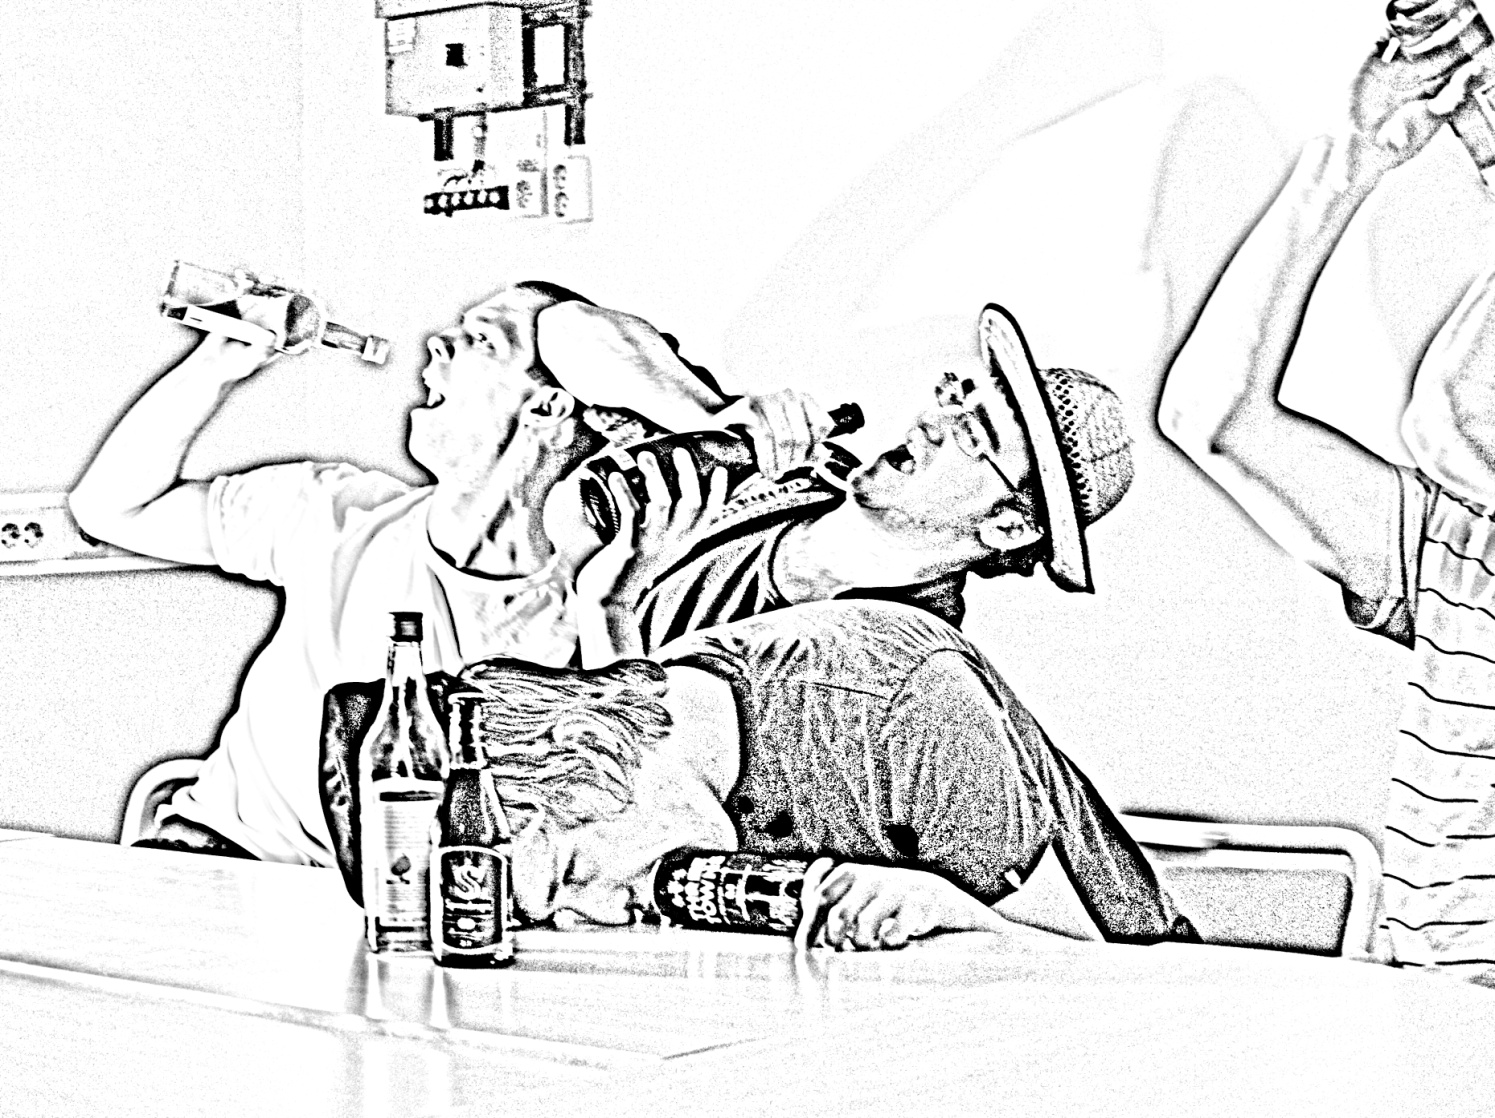
\includegraphics[width=1.0\textwidth]{res/bordsvisor.png}
   \section{Bordsvisor}
   
\end{center}
\vfill
\newpage


\subsection{Måltidssång (Fredmans epistel nr 21)}
\index[alfa]{Måltidssången (Fredmans epistel nr 21)}
\index[anfa]{Så lunka vi så småningom...}
\textit{Mel: Måltidssång\\skriven av Carl Michael Bellman}\\
\begin{parse lines}[\noindent]{#1\\}

Så lunka vi så småningom
från Bachi buller och tumult.
När döden ropar: Granne, kom,
ditt timglas är nu fullt!
Du gubbe fäll din krycka ner
och du, du yngling lyd min lag:
Den skönsta nymf som åt dig ler
inunder armen tag!

Tycker du att graven är för djup?
Nå, välan, så tag dig då en sup!
Tag dig sen dito en, dito två, dito tre;
så dör du nöjdare.

Säg, är du nöjd, min granne, säg?
Så prisa världen nu till slut!
Om vi har en och samma väg
så följoms åt... Drick ut!
Men först med vinet, rött och vitt,
för vår värdinna bugom oss,
och halkom sen i graven fritt
vid aftonstjärnans bloss!

Tycker du…
\end{parse lines}


\subsection{Fyllevisa}
\textit{Mel: Vi gå över daggstänkta berg}\\
\index[alfa]{Fyllevisa}
\index[anfa]{Vi som oss för att glupa satt...}
\begin{parse lines}[\noindent]{#1\\}

Vi som oss för att glupa satt
supa glatt,
ity den, som försmår sin första tår
törsta får.
Av längtan vi tryckas
av trängtan att lyckas.
Vi nu med bravur häller ur, eller hur?

Vi ger titt som tätt strupen sitt: 
Supen stritt
skall forsa, och snart får sig tarmen vår
varm en tår. 
Er öven i seder och söven sen ned er
vid denna protest-bullerfest: Full är bäst!
\end{parse lines}
\vspace{-0.2cm}
\subsection{Köttet kommer}
\textit{Mel: Vals ur Glada Änkan}\\
\index[alfa]{Köttet kommer}
\index[anfa]{Köttet kommer, köttet kommer mört och rött...}
\begin{parse lines}[\noindent]{#1\\}

Köttet kommer, köttet kommer mört och rött.
Gnäggar inte springer inte, det är dött.
Skål för alla oxar! Skål för varje säl.
Skål för alla hästar som vi slått ihjäl!

Raj raj raj raj raj... 
\end{parse lines}
\newpage

\subsection{Spritbolaget}
\textit{Mel: Du käre lille snickerbo}\\
\textit{Sångarstriden 1989}\\
\index[alfa]{Spritbolaget}
\index[anfa]{Till spritbolaget ränner jag...}
\begin{parse lines}[\noindent]{#1\\}

Till spritbolaget ränner jag
och bankar på dess port.
Jag vill ha nåt som bränner bra
och gör mig sketfull fort.
Expediten sade: Godda',
hur gammal kan min herre va?
Har du nåt leg, ditt fula drägg?
Kom hit igen när du fått skägg!

Nej, detta var ju inte bra,
jag ska bli full ikväll.
Då plötsligt en idé fick jag:
De har ju sprit på Shell.
Många flaskor stod där på rad,
så nu kan jag bli full och glad.
Den röda drycken åkte ner...
Nu kan jag inte se nåt mer
\end{parse lines}

\newpage

\subsection{Lackalänga}
\textit{Mel: Horgalåten}\\
\textit{Skriven av Inspektor Jan Eric Larsson}\\
\index[alfa]{Lackalänga}
\index[anfa]{Uti Lackalänga är det sorgeligt...}
\begin{parse lines}[\noindent]{#1\\}

Uti Lackalänga är det sorgeligt,
där är det sorgeligt,
där stänger kiosken tidigt.

Uti Lackalänga är det sorgeligt,
där är det sorgeligt,
där är det stängt.

Men i Åstorp, men i Åstorp,
där är kiosken öppen natten lång.

Men i Åstorp, men i Åstorp,
där är kiosken öppen natten lång.

Uti Lackalänga är det sorgeligt,
där är det sorgeligt,
där är det stängt.

\end{parse lines}

\newpage
\subsection{Skotten}
\textit{Mel: Scotland brave}\\
\index[alfa]{Skotten}
\index[anfa]{Jag kommer ifrån Skottland...}
\begin{parse lines}[\noindent]{#1\\}

Jag kommer ifrån Skottland.
Det är ett kallt och rått land.
Nu bor jag uti London,
som ni kan se på fonden.

Mitt liv är ganska riskigt;
jag dricker sliskig whisky,
och när som kilten faller
är rumpan bar.
\end{parse lines}


\subsection{Härjarevisan}
\textit{Mel: Gärdebylåten}\\
\textit{ur Djingis Khan-spexet 1954}\\
\index[alfa]{Härjarevisan}
\index[anfa]{Hurra"! Nu ska man äntligen få röra på benen...}
\begin{parse lines}[\noindent]{#1\\}

Hurra! Nu ska man äntligen få röra på benen.
Hela stammen jublar och det spritter i grenen.
Tänk, att än en gång få spränga 
fram på Brunte i galopp!
Din doft, o kära Brunte, är, trots brist i hygienen,
för en vild mongol minst lika ljuv som syrenen.
Tänk, att på din rygg få rida runt
i stan och spela topp!Ja, för nu ska vi ut och härja,
supa och slåss och svärja,
bränna röda stugor, slå små barn
och säga fula ord.
Med blod ska vi stäppen färga;
nu änteligen lär jag kunna
dra nån riktig nytta
av min Hermodskurs i mord.

Ja, mordbränder är klämmiga, ta fram fotogenen!
Eftersläckningen tillhör just de fenomenen
inom brandmansyrket som jag tycker
det är nån nytta med.
Jag målar för mitt inre upp den härliga scenen:
blodrött mitt i brandgult. Ej ens prins Eugen en
lika mustig vy kan måla, 
ens om han målade med sked.

Ja, för nu ska vi ut och härja...
\end{parse lines}

\newpage
\subsection{Jag har aldrig varit på snusen}
\textit{Mel: O hur saligt att få vandra}\\
\index[alfa]{Jag har aldrig varit på snusen}
\index[anfa]{Jag har aldrig vatt på snusen...}
\begin{parse lines}[\noindent]{#1\\}

Jag har aldrig vatt på snusen,
aldrig rökat en cigarr - halleluja!
Mina dygder äro tusen,
inga syndiga laster jag har.

Jag har aldrig sett nåt naket,
inte ens ett litet nyfött barn.
Mina blickar går mot taket,
därmed undgår jag frestarens garn.

Halleluja...

Bachus spelar på gitarren,
Satan spelar på sitt handklaver.
Alla djävlar dansar tango,
säg vad kan man väl önska sig mer?

Jo, att alla bäckar vore brännvin,
stadsparksdammen full av bayerskt öl,
konjak i varenda rännsten
och punsch i varendaste pöl.

Och mera öl... 
\end{parse lines}


\subsection{Vikingen}
\textit{Mel: When Johnny comes marching home}\\
\textit{E-sektionen Sångarstriden 1981}\\
\index[alfa]{Vikingen}
\index[anfa]{En viking vill ha livets vann...}
\begin{parse lines}[\noindent]{#1\\}

En viking vill ha livets vann,
hurra, hurra! 
Den hastigt i mitt svalg försvann,
hurra, hurra! 
Till kalv, till oxe, till fisk, till fläsk, 
när somliga bara dricker läsk,
då vill alla sanna vikingar ha en bäsk. 

När vi druckit bäsken slut,
tragik, tragik!
Då bäres varje viking ut,
som lik sig lik.
Och sen, om vi vaknar, vi sjunger en bit, 
sen korkar vi upp Skånes akvavit.
Skål för alla vikingar som kom hit!
\end{parse lines}

\newpage
\subsection{Mobiltelefonen}
\textit{Mel: Min hatt den har tre kanter}\\
\textit{Lundakarnevalen 2006}\\
\index[alfa]{Mobiltelefonen}
\index[anfa]{Min Sony har en kamera...}
\begin{parse lines}[\noindent]{#1\\}

Min Sony har en kamera,
en dator och kompass.
Men den har ingen korkskruv,
Det tycker jag är kasst!
\end{parse lines}


\subsection{På golvet}
\textit{Mel: Dotter Sion}\\
\index[alfa]{På golvet}
\index[anfa]{Flaskan på bordet...}
\begin{parse lines}[\noindent]{#1\\}

Flaskan på bordet
tömdes i en väldig fart
Men att varva den med vatten
är helt otänkbart

Snart så kryper vi på golvet
Och samtalar med skor
Träffar på en trevlig socka
Ser det är min bror

Nyss var det flaskan
nu är jag den som är full
När jag tar dess plats på bordet
trillar vi omkull
\end{parse lines}


\subsection{Det naturliga urvalet}
\textit{Mel: Skånska slott och herresäten}\\
\index[alfa]{Det naturliga urvalet}
\index[anfa]{När Darwin studerade liv i naturen...}
\begin{parse lines}[\noindent]{#1\\}

När Darwin studerade liv i naturen
Så fann han att först dör de svagaste djuren
De sämsta bland hjärnceller dör också först
Så öka din IQ och minska din törst

När Einstein studerade massan och ljuset
så ljusnade plötsligt problemet med ruset:
ett glas med en hel massa renat uti
förvandlas i kroppen till ren energi.
\end{parse lines}

\newpage
\subsection{Jag har aldrig varit i frysen}
\textit{Mel: O hur saligt att få vandra}\\
\index[alfa]{Jag har aldrig varit i frysen}
\index[anfa]{Jag har aldrig vart i frysen...}
\begin{parse lines}[\noindent]{#1\\}

Jag har aldrig vart i frysen
Aldrig frusit ens en pall - halleluja
Mina grader äro tusen
Inga djupfrysta glassar jag tar

Jag har aldrig sett nåt fruset
inte ens ett litet nedkylt barn
Mina lågor värmer huset
därmed undgår jag köldmediets garn

Halleluja…

Kelvin spelar på gitarren
Satan fryser ner sitt högkvarter
Alla djävlar dricker kväve
säg vad kan man väl önska sig mer?

Jo, att alla bäckar vore iste
stadsparkdammen täckt med inlandsis
konjak i vartenda frysfack
och köld i varendaste spis

Vomera is...
\end{parse lines}


\subsection{Dessertvisa}
\textit{Mel: Sjösala vals}\\
\index[alfa]{Dessertvisa}
\index[anfa]{Gästerna de springer i pausen på dass...}
\begin{parse lines}[\noindent]{#1\\}

Gästerna de springer i pausen på dass,
eftersom de fyllt sina magar så pass.
Maten den har smakat, 
jag har tatt flera lass,
men vet att nu nalkas det 
hjortron och glass!

Kurre, kurre kurre, 
min mage känns så stinn.
Jag ångrar nu så bittert 
att jag har spänt mitt skinn.
Men banta kan jag glömma, 
det är ju finsittning det här!
Bältet jag spänner upp, 
gör plats för mer dessert!
\end{parse lines}

\newpage
\subsection{Jag vill ut och gasqua}
\textit{Mel: You can’t get a man with a gun}\\
\index[alfa]{Jag vill ut och gasqua}
\index[anfa]{Jag vill ut och gasqua"!}
\begin{parse lines}[\noindent]{#1\\}

Jag vill ut och gasqua!
Var fan är min flaska?
Vem i helvete stal min butelj?
Skall mej törsten betvinga?
En TT börja svinga?
Nej för fan bara blunda och svälj!
Vilken smörja!
Får jag spörja?
Vem för fan tror att jag är en älg?

Till England vi rider,
och sedan vad det lider
träffar vi välan på någon PUB.
Och där ska vi festa!
Blott dricka av det bästa
utav whiskey och portvin.
Jag tänker gå hårt in
för att prova på rubb och stubb.
\end{parse lines}

\newpage

\subsection{Lyft ditt välförsedda glas}
\textit{Mel: Ding dong merrily on high}\\
\index[alfa]{Lyft ditt välförsedda glas}
\index[anfa]{Lyft ditt välförsedda glas...}
\begin{parse lines}[\noindent]{#1\\}

Lyft ditt välförsedda glas
Det är en härlig börda
Nu har grabbarna kalas
Vi segern snart skall skörda
$\vert\vert$: Ding dingedingeding dingedingeding
dingedingeding dong dong
Imorgon är det lördag. :$\vert\vert$

Sätt nu glaset till din mun
Se döden på dig väntar
Nu har grabbarna kalas
Hör liemannen flämtar
$\vert\vert$: Ding dingedingeding dingedingeding
dingedingeding dong dong
Begravningsklockor klämtar. :$\vert\vert$
\end{parse lines}

\newpage
\subsection{Jag har aldrig varit på UB}
\textit{Mel: O hur saligt att få vandra}\\
\textit{E-sektionen Sångarstriden 2009}\\
\index[alfa]{Jag har aldrig varit på UB}
\index[anfa]{aldrig pluggat på Café Athen...}

\begin{parse lines}[\noindent]{#1\\}
Jag har aldrig varit på UB,
aldrig pluggat på Café Athen,
aldrig skurit upp en snubbe,
kan ej skilja artär från ven.

Jag har aldrig börjat klockan 9,
eller slutat 14:32.
I AF-borgen går jag vilse,
för jag går på LTH.

Dom har aldrig vart på ön Øn,
aldrig målat Väg och Vattens spik.
Aldrig haft det stora nöjet,
att få somna till Böijers logik.

Dom har aldrig vunnit en Regatta,
eller festat i en skitig ouveralle.
Aldrig däckat bakom Lophtet,
för dom går ej på LTH.

E kan j-omega och Ohms lag.
F och Nano fattar kvantfysik.
Eko, eko, eko, eko,
eko, eko med akvatik.

I och M kan ragga på kemister.
Data knackar på sin kära linuxkod.
Inga här är humanister,
för vi är alla LTH

I och M kan ragga på kemister.
Data knarkar på sin kära linuxkod.
Mardrömmar om humanister,
drömmer alla på LTH.
\end{parse lines}


\subsection{Kissemiss}
\textit{Mel: She’ll be coming ’round the mountain}\\
\index[alfa]{Kissemiss}
\index[anfa]{Tänk så trevligt att ni kunde komma hit...}
\begin{parse lines}[\noindent]{#1\\}

Tänk så trevligt att ni kunde komma hit
Låt oss ta en liten jamare med flit
Blir vi sedan lätt i hatten,
ja då kan man ge sig katten
på att jamaren vi tatt den var av sprit.
Så sjung mjau, mjau, kissemisse mjau
Ja, sjung mjau, mjau, kissemisse mjau
Om vi jamar hela natten
desto gladare blir skratten
efter slatten får rabatten en visit. 
\end{parse lines}


\begin{picture}(50,50) \put(150,-45){\hbox{
\includegraphics[scale=0.35]{res/katt.png}}} \end{picture}


\newpage
\subsection{Jag ska festa}
\vspace{-0.1cm}
\textit{Mel: Bamse}\\
\textit{D-sektionen Sångarstriden 1987}\\
\vspace{-0.1cm}
\index[alfa]{Jag ska festa}
\index[anfa]{Jag ska festa, ta det lugnt med spriten...}
\begin{parse lines}[\noindent]{#1\\}

Jag ska festa, ta det lugnt med spriten,
ha det roligt utan å va full.
Inte krypa runt med festeliten,
ta det varligt för min egen skull

Först en öl i torra strupen,
efter det så kommer supen,
i med vinet, ner med punschen.
Sist en groggbuffé.

Jag är skitfull, däckar först av alla,
missar festen, men vad gör väl de?
Blandar hejdlöst öl och gammal filmjölk,
kastar upp på bordsdamen breve!

Sen en öl...

Spyan rinner ner för ylleslipsen.
Raviolin torkar i mitt hår.
Vem har lagt mig under matsalsbordet?
Vems är gaffeln i mitt högra lår?

Sist en öl...
\end{parse lines}

\noindent\textit{Originalet slutar efter andra versen.
Sista versen har tillkommit senare.}




\subsection{Stopp en stund}
\textit{Mel: Räven raskar över isen}\\
\index[alfa]{Stopp en stund}
\index[anfa]{Stopp en stund med skratt och pratet...}
\begin{parse lines}[\noindent]{#1\\}

Stopp en stund med skratt och pratet,
kniv och gaffel lägg på fatet.
Seden är, att så här,
man handskas med destilatet.

Man lyfter glaset med höger hand,
och trycker läpparna mot dess rand.
Man dricker ur, och grinar sur,
och väntar på resultatet.

\end{parse lines}




\subsection{Treo-comp}
\textit{Mel: Längtan till landet}\\
\index[alfa]{Treo-comp}
\index[anfa]{Morgonstund med smak av döda bävrar...}
\begin{parse lines}[\noindent]{#1\\}

Morgonstund med smak av döda bävrar 
frukostmorgonen är över oss 
hur vi alla stretar, hur vi vägrar 
så går solen lik förbannat opp

Snart är dagen här med hemska plågor 
huvudvärk, yrsel, elände men 
det finns faktiskt ett glas som dej kan rädda 
Treo-comp vår frälsare och vän.
\end{parse lines}

\subsection{Törsten rasar}
\textit{Mel: Längtan till landet}\\
\index[alfa]{Törsten rasar}
\index[anfa]{Törsten rasar uti våra strupar...}
\begin{parse lines}[\noindent]{#1\\}

Törsten rasar uti våra strupar,
tungan hänger torr och styv och stel.
Men snart vankas stora, kalla supar,
var och en får sin beskärda del.

Snapsen kommer, den vi vilja tömma,
denna nektar lik Olympens saft,
kommer oss att våra sorger glömma.
Snapsen skänker hälsa, liv och kraft.

Fordom odlade man vindruvsranka,
av vars frukt man gjorde ädelt vin.
Nu man pressar saften ur en planka,
doftande av äkta terpentin.

Höj din bägare, O, Broder, yster,
och låt svenska skogen glida kall,
ner för strupen och om sen det dig lyster,
låt oss supa opp en liten tall.

Helan tänder helig eld i själen,
halvan rosar livet som en sky.
Tersen känns från hjässan ner i hälen,
kvarten gör oss till en mänska ny.

Låt oss skåla med varann, go’ vänner,
skål för våran levnads glada lopp,
törstens eld på nytt i strupen bränner.
Leve livet! Skål och botten opp!
\end{parse lines}







\vspace{-0.5cm}
\subsection{När jag kissar överallt}
\textit{Mel: Skånska slott och herresäten}\\
\textit{Lundakarnevalen 1986}\\
\index[alfa]{När jag kissar överallt}
\index[anfa]{På gator som trampats av Ask och von Platen...}
\begin{parse lines}[\noindent]{#1\\}

På gator som trampats av Ask och von Platen 
På stenar som blickat på Broman, Piraten 
På Lundagårds träd som har skuggat Tegnér 
På allt har jag kissat och lustfyllt blött ner

\textit{Sjunges med ett långt s-ljud efter varje rad för att simulera urinering.}

\end{parse lines}

\vspace{-0.9cm}
\subsection{Gamla vänner}
\textit{Mel: My darling Clementine}\\
\index[alfa]{Gamla vänner}
\index[anfa]{Gamla vänner, vi som känner...}
\begin{parse lines}[\noindent]{#1\\}

Gamla vänner, vi som känner,
att vår ungdoms ork finns kvar:
Lyft pokalen här i salen,
till en skål för flydda dar.

O vår ungdom, glada ungdom,
ta din bägare i hand.
Skål för alla som här tralla,
skål för gamla vänskapsband.
\end{parse lines}


\vspace{-1cm}
\subsection{För en lyckad kväll}
\textit{Mel: Twelve days of christmas}\\
\textit{Bordsvisa D-sektionen 2010}\\
\index[alfa]{För en lyckad kväll}
\index[anfa]{För en trevlig kväll packar jag ner några öl...}
\begin{parse lines}[\noindent]{#1\\}

För en trevlig kväll packar jag ner några öl
- och en shot för en lyckad kväll

Jag kommer till min förfest och bjuds snabbt på en drink:
- en Red Bull-vodka
- och en shot för en lyckad kväll

Folk skriker LAMBO och jag ställs upp på en stol:
- två burkar öl
- en Red Bull-vodka
- och en shot för en lyckad kväll

Jag vinglar mot nationen o humöret är på topp:
- delar bag-in-box
- två burkar öl
- en Red Bull-vodka
- och en shot för en lyckad kväll


Blir vägrad av vakten men finner till min tröst:
- en flaska rom
- delar bag-in-box
- två burkar öl
- en Red Bull-vodka
- och en shot för en lyckad kväll

Jag spyr i närmsta buske och finner vad som gömts:
- tre fulla cider
- en flaska rom
- delar bag-in-box
- två burkar öl
- en Red Bull-vodka
- och en shot för en lyckad kväll

Jag vaknar dagen efter och hittar bredvid mig:
- ett äckligt hemsläp
- tre fulla cider
- en flaska rom
- delar bag-in-box
- två burkar öl
- en Red Bull-vodka
- och en shot från en lyckad kväll
\end{parse lines}

\newpage


\subsection{Hundmat}
\textit{Mel: Man ska ha husvagn}\\
\textit{D-sektionen Sångarstriden 1990}\\
\index[alfa]{Hundmat}
\index[anfa]{Att va student är nåt som inte alltid är så lätt...}
\begin{parse lines}[\noindent]{#1\\}

Att va student är nåt som inte alltid är så lätt.
Man måste spara pengar och man måste äta rätt.
När pengarna är slut och alla kläder är i pant,
då har jag kommit på hur man kan spara sig en slant.

Jag äter hundmat, när hushållskassan gått i sin.
Jag äter hundmat, och klarar av ekonomin.
Jag äter hundmat, det kan va lagat eller rått.
Jag äter hundmat, åsså är det gott.

Men vänner har jag inga kvar – 
förutom grannens jycke.
Vi brukar äta ute och vi delar varje stycke,
Och bjuder nån på middag
tar jag hem i doggybag,
men tar nån skålen från mig 
blir jag arg och reser ragg.

Jag äter hundmat, med läckert kycklingkött i bit.
Jag äter hundmat, och Frolic är min favorit.
Jag äter hundmat, det passar bra när man är pank. 
Jag äter hundmat, och pälsen den blir blank.

Ge mig Frolic och en klapp, eller lite Chappi.
Mycket näring finns i Snap, Caesar gör mig happy.
Ge mig Schmackos, torkat kött, ge mig lite Pal.
Vov är bra när man är trött men godast är Royal.

Jag äter hundmat, jag stoppar ner det i min tarm.
Jag äter hundmat, behöver inte vara varm.
Jag äter hundmat, och jag blir mätt och glad och fin.
Jag äter hundmat, bra med protein.

Jag äter hundmat, för den är full med nyttigt kött.
Jag äter hundmat, gjord på råtta som har dött.
Jag äter hundmat, min vovve går med magen tom.
Jag äter hundmat, billig mat från Dogman i min gom.
\end{parse lines}

\newpage
\subsection{Ode till Aq-va-kul}
\textit{Mel: Till glädjen}\\
\textit{Bordsvisa D-sektionen 2008}\\
\index[alfa]{Ode till Aq-va-kul}
\index[anfa]{Likt en nedkyld öl vi svettas...}
\begin{parse lines}[\noindent]{#1\\}

Likt en nedkyld öl vi svettas
törstiga i Malmö stad
nu ska vi av spriten tvättas,
fyller upp ett alkisbad

Grunden är försvagad - men ärligt:
inför en kväll i akvavit
underhållet kvittar när vi
kastat oss i klorad sprit

Efter många kallsupar har
snart hela bassängen tömts
Festen den har nått till botten
där den sista tåren gömts. 

Dyker ner för sista skålen 
höjer mitt glas med simmig blick
kisar mot de stora hålen
är i ganska dåligt skick.

Ner i magen rutschar nu slatten
alla bekymmer spolas bort 
Vi har skoj med livets vatten.
Aqua-kul det river gott
\end{parse lines}


\subsection{Vit vecka}
\textit{Mel: White Christmas}\\
\index[alfa]{Vit vecka}
\index[anfa]{Jag drömmer om en vit vecka...}
\begin{parse lines}[\noindent]{#1\\}

Jag drömmer om en vit vecka.
Sju dagar utan alkohol.
Tänk att bara skåla i juice och Cola och sedan minnas allt man gjort.

Jag drömmer om en vit vecka, 
det finns en gräns för vad jag tål.
Jag vill inte dricka mera sprit så låt nästa vecka vara vit.
\end{parse lines}


\subsection{Uti min mage}
\textit{Mel: Uti vår hage}\\
\index[alfa]{Uti min mage}
\index[anfa]{Uti min mage en längtan mig tär...}
\begin{parse lines}[\noindent]{#1\\}

Uti min mage en längtan mig tär,
kom hjärtans fröjd.
Där råder en hunger som ropar så här:
Kom kryddsill och kall potatis,
kom ostar och quantum satis,
kom allt som kan ätas,
kom hjärtans fröjd.
\end{parse lines}

\newpage
\subsection{Jesus lever}
\textit{Mel: Sånt är livet}\\
\index[alfa]{Jesus lever}
\index[anfa]{Jesus lever, han bor i Skövde...}
\begin{parse lines}[\noindent]{#1\\}

Jesus lever, han bor i Skövde
Han kör en Volvo och han är gift
Han har en villa med rododendron
Han sparar pengar och jobbar skift

Redan på lekis var han märklig
Han ville inte leka krig
Men när hans kompis, Knut, blev skjuten
så lät han Jesus uppväcka sig

Jesus lever, han bor i Skövde...

Han gick i skolan, som alla andra
Han var rätt duktig på gymnastik
å vilken kille han gick på vatten
en gång så gick han till Reykjavik

Jesus lever, han bor i Skövde...

I sina tonår så var han poppis
Och han blev bjuden på varje fest
Å vilken kille, han fick ju vatten
att bli till rusdryck utan jäst

$\vert\vert$: Jesus lever, han bor i Skövde... :$\vert\vert$
\end{parse lines}


\subsection{Spela Skyrim}
\textit{Mel: Dragonborn}\\
\textit{Skriven av Axel Hellman}\\
\index[alfa]{Spela Skyrim}
\index[anfa]{Ner med vin, mera vin...}
\begin{parse lines}[\noindent]{#1\\}

Ner med vin, mera vin
lite punsch gör mig fin
Välter öl, spiller sprit
gjordes inte med flit

Häver upp i en säck, tredje dagen i sträck
Vaknar upp bredvid någon som jag aldrig har sett

Utbringa skål! JA!
Hörde jag dubbel skål? JA!
\end{parse lines}
\vfill
\noindent\textit{Kom på andraplats under bordsvisesittningen 2015 och har sedan dess envist skickats in och sjungits varje år.}

\newpage
\subsection{Baklängesfyllan}
\textit{Mel: Rövarna i Kamomilla stad}\\
\textit{Vinnande övrig visa, Lundakarnevalen 2018}\\
\index[alfa]{Baklängesfyllan}
\index[anfa]{Jag hulkar i mig spyorna...}
\begin{parse lines}[\noindent]{#1\\}

Jag hulkar i mig spyorna, 
och sedan med en gaffel, 
ur munnen min jag plockar fram, 
en extra stor falafel. 

Sen baklänges jag vinglar bort, 
till efterfest av bästa sort. 
Jag spottar ut shot, efter shot, efter shot 
ja så här finemang har jag aldrig mått! 

(Å shot, shot, shot, shot. Å shot, shot, shot, shot.) 

Till Lundagård jag rullar sen, 
och ställer någons cykel. 
På klubbens dansgolv hittar jag. 
min plånbok och min nyckel. 

Fem öl, sju snaps, en flaska vin, 
jag häller upp ur halsen min. 
Ikväll ska jag plugga det lovar jag dig, 
men en endaste öl kan man unna sig!
\end{parse lines}

\subsection{Tenta efter jul}
\textit{Mel: Mössens julafton}\\
\textit{Vinnande bidrag bordsvisesittning 2017}\\
\index[alfa]{Tenta efter jul}
\index[anfa]{När julen börjar närmas...}
\begin{parse lines}[\noindent]{#1\\}

När julen börjar närmas
och man vill koppla av
Så kommer tentaplugget
här och ställer sina krav

Jag börjar kompromissa
gör julrimmen i C
Försöker strukturera
pluggar fram till klockan tre

Programmering lin-jär algebra
Endim å reglerteknik är ingenting att ha
Tenta efter nyår är ju trist
Men skippar man för många ja då blir man alkolist

Skål!
\end{parse lines}
\vfill
\noindent\textit{Skrevs på 45 minuter medan sittningen riggades.}

\newpage
\subsection{O gamla klang och jubeltid}
\textit{Mel: O alte Burschenherrlichkeit}\\
\index[alfa]{O gamla klang och jubeltid}
\index[anfa]{O, gamla klang och jubeltid...}
\begin{parse lines}[\noindent]{#1\\}

O, gamla klang och jubeltid,
ditt minne skall förbliva,
och än åt livets bistra strid
ett rosigt skimmer giva.
Snart tystnar allt vårt yra skämt,
vår sång blir stum, vårt glam förstämt;
o, jerum, jerum, jerum,
o, quae mutatio rerum!

Var äro de som kunde allt,
blott ej sin ära svika,
som voro män av äkta halt
och världens herrar lika?
De drogo bort från vin och sång
till vardagslivets tråk och tvång;
o, jerum, jerum, jerum,
o, quae mutatio rerum!

Den ene vetenskap och vett
in i scholares mänger,
den andre i sitt anlets svett
på paragrafer vränger,
en plåstrar själen som är skral,
en lappar hop dess trasiga fodral;
o, jerum, jerum, jerum,
o, quae mutatio rerum!

Men hjärtat i en sann student
kan ingen tid förfrysa.
Den glädjeeld, som där han tänt,
hans hela liv skall lysa.
Det gamla skalet brustit har,
men kärnan finnes frisk dock kvar,
och vad han än må mista,
den skall dock aldrig brista.

Så sluten, bröder, fast vår krets
till glädjens värn och ära!
Trots allt vi tryggt och väl tillfreds
vår vänskap trohet svära.
Lyft bägarn högt och klinga, vän!
De gamla gudar leva än
bland skålar och pokaler,
bland skålar och pokaler!
\end{parse lines}

\newpage

\subsection{Whiskey ur kastrull}
\textit{Mel: Whiskey in the Jar}\\
\textit{Skriven av Lukas Lönnborn}\\
\index[alfa]{Whiskey ur kastrull}
\index[anfa]{Jag vakna härrom morra...}

\begin{parse lines}[\noindent]{#1\\}
Jag vakna härrom morra
upp och ner i sängen
Jag slängde mig på cykeln
och jag slirade i svängen

Det hade ryktats om en förfest
Jag sträckte ena muskeln
Jag stannade vid delphi
kasta cykeln min i busken

$\vert\vert$: Och sa: tjofaddelittanlej
och finns det inga glas
på detta förkalas
drick vodka ur en vas :$\vert\vert$

På delphi gick jag vilse
som alla andra
Jag träffa en blonderad tjej
hon sa hon hette Sandra

Hon var också vilse
och hade gråten sin i halsen
jag trösta na med spritbolaget
satte hela svansen


$\vert\vert$: Och sa: tjofaddelittanlej
Hitåt, det är min tes
Nä jag är ingen mes
drick ouzo ur en fez :$\vert\vert$

När vi hitta festen
så var folket borta
men dörren den stod vidöppen
gick in med stegen korta

Och på bordet där stod spriten
som blitt över från förfesten
jag tittade på Sandra sa:
"Nu dricker vi upp resten!"

$\vert\vert$: Och hon sa: tjofaddelittanlej
Och fastän jag är full
Jag super dig omkull
drick whiskey ur kastrull :$\vert\vert$

Någonstans i dimman
Finns ett litet minne
Från när vi supt ihjäl varann
Ja, väck från själ och sinne

På golvet låg en orm
“Sandra, titta där”
Hon tog tag i ormen
Det var en öldrickarmackapär

$\vert\vert$: Och jag sa: tjofaddelittanlej
Nu sätter vi igång
Med ett jävla fjong
Drick bira ur en bong :$\vert\vert$

När vi skiljdes åt
Jag vet ej var hon gick hänn
Men det spelar faktiskt ingen roll
Jag hade en ny vän

Sen så gick jag hem
jag åt en liter Sia
Och tog en återställare
blanda filmjölk med sangria

$\vert\vert$: Och sa: tjofaddelittanlej
vad gör man då måntro
för att den ska va’ go’
drick upp den ur en sko :$\vert\vert$

Jag vakna nästa morra
upp och ner i sängen
jag slängde mig på cykeln
och jag slirade i svängen
\end{parse lines}
\vfill
\noindent\textit{Framfördes ursprungligen med tre verser inför \linebreak sångförmansvalet på HTM-Val 2017.}

\newpage
\thispagestyle{empty}
\null
\vfill
\begin{center}

   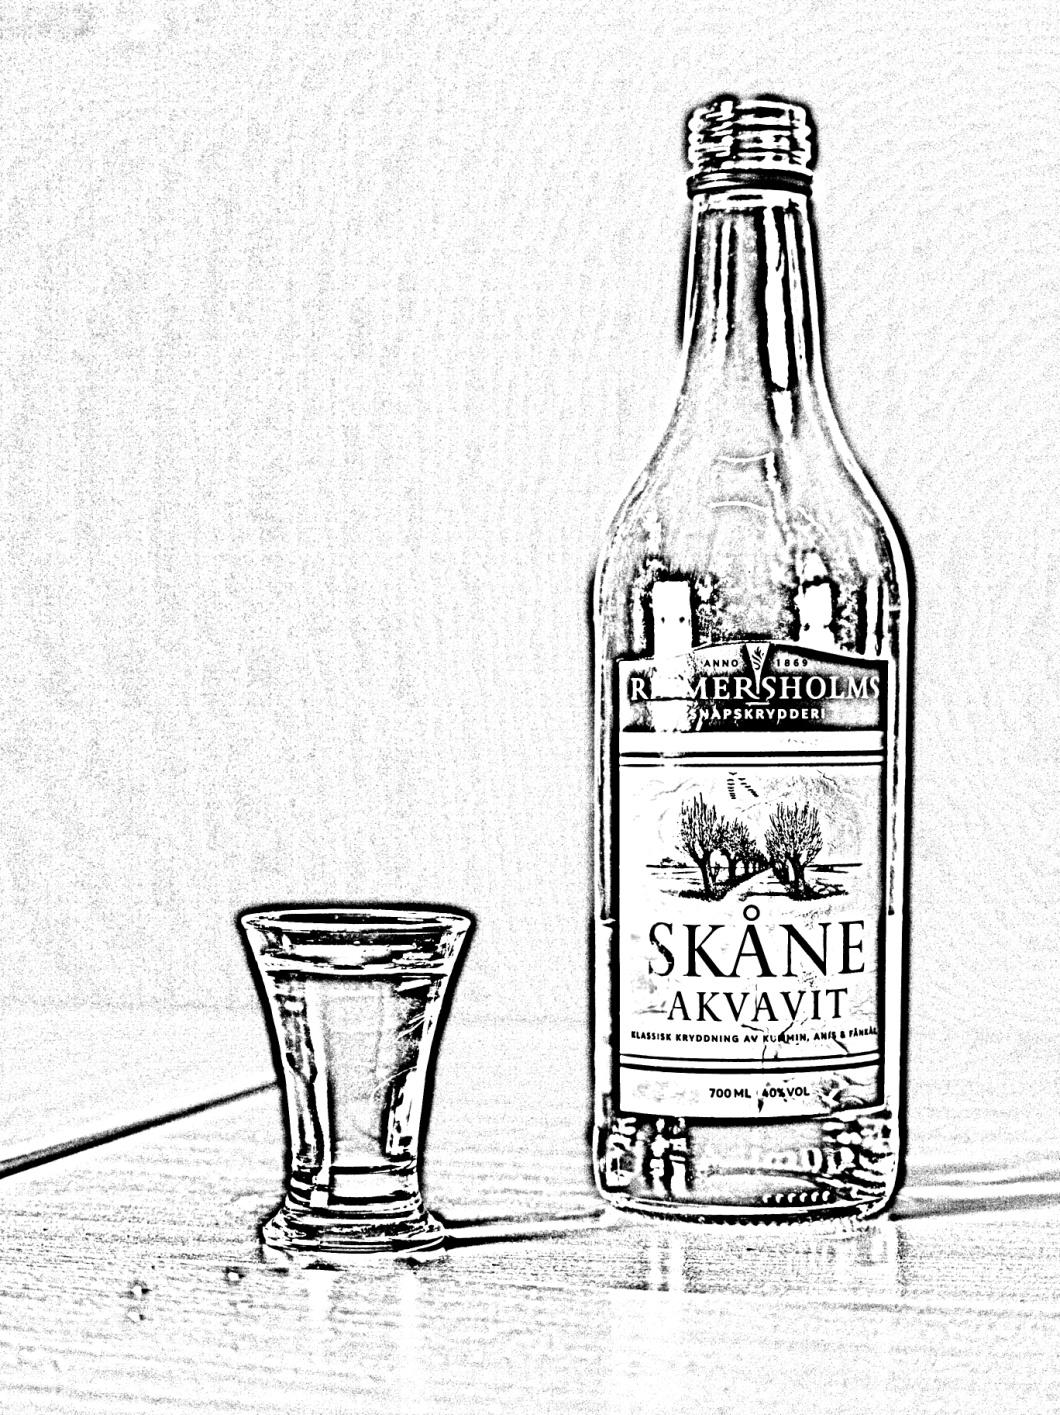
\includegraphics[width=0.8\textwidth]{res/snapsvisor.jpg}
   \section{Snapsvisor}
   
\end{center}
\vfill
\newpage

\subsection{1, 2, 75, 6, 7}
\textit{Mel: Ritsch, ratsch}\\
\index[alfa]{1, 2, 75, 6, 7}
\index[anfa]{1, 2, 75, 6, 7, 75...}
\begin{parse lines}[\noindent]{#1\\}

1, 2, 75, 6, 7, 75, 6, 7, 75, 6, 7,
1, 2, 75, 6, 7, 75, 6, 7, 73,
107, 103, 102, 107, 6, 19, 27,
17, 18, 16, 15, 13, 19, 14, 17,
19, 16, 18, 11, 8, 47.
\end{parse lines}

\subsection{Mera brännvin}
\textit{Mel: Internationalen}\\
\index[alfa]{Mera brännvin}
\index[anfa]{Mera brännvin i glasen...}
\begin{parse lines}[\noindent]{#1\\}

Mera brännvin i glasen,
mera glas på vårt bord,
mera bord på kalasen,
mer kalas på vår jord.

Mera jordar med måne,
mera månar i mars,
mera marscher till Skåne,
mera Skåne, Gud bevars, bevars, bevars!
\end{parse lines}

\newpage
\subsection{75:an}
\textit{Mel: 34:an}\\
\index[alfa]{75:an}
\index[anfa]{Våra tentor har vi flunkat...}
\begin{parse lines}[\noindent]{#1\\}

Våra tentor har vi flunkat
Vi har fått vår diagnos
Nu vår HB vi har dunkat
Vi ska hamna i hypnos
Det gör inget om det luktar
Som en flaska med klorin
För vi ska ju bara fukta
Våra läppar med vårt vin

Men sen är det slut på fina viner
Ja, nu ska vi korka upp vår sprit
Det ska halsas utav OP
Absolut och akvavit
Ja, jag tar farväl av hjärnans celler
Vaknar aldrig mer
Nu är det slut på fina viner
Nu ska sjuttifemman i magen ner!
\end{parse lines}

\newpage
\subsection{Änglahund}
\textit{Mel: Marseljäsen}\\
\textit{Sångarstriden 1991}\\
\index[alfa]{Änglahund}
\index[anfa]{Det står en hund på fjärde våningen...}
\begin{parse lines}[\noindent]{#1\\}

Det står en hund på fjärde våningen,
och den tänker hoppa ner.

BANZAÏ!

Det var en japanesisk självmordshund,
och den hoppar aldrig mer.
\end{parse lines}

\subsection{Armen i vinkel}
(Ramsa)\\
\index[alfa]{Armen i vinkel}
\index[anfa]{Armen i vinkel...}
\begin{parse lines}[\noindent]{#1\\}

Armen i vinkel,
blicken i skyn.
Så var det menat,
whisky och renat.
Vårt mål: alkohol,
skål för den som tål, SKÅL!
\end{parse lines}

\newpage
\subsection{Att fela är mänskligt}
\textit{Mel: Prästens lilla kråka}\\
\textit{Lundakarnevalen 2010}\\
\index[alfa]{Att fela är mänskligt}
\index[anfa]{Trampa på ett smådjur...}
\begin{parse lines}[\noindent]{#1\\}

Trampa på ett smådjur,
slakta gulligt rådjur,
måste göras rätt försiktigt...

Gifta sig med släkten,
stjäla ur kollekten,
det är FEL och det är viktigt!

$\vert\vert$: Men att sjunga en snutt,
och ta sig en hutt - 
Det är bara RÄTT och riktigt! :$\vert\vert$
\end{parse lines}


\subsection{Dricka långsamt}
\textit{Mel: Här kommer Pippi Långstrump}\\
\index[alfa]{Dricka långsamt}
\index[anfa]{Visst kan man dricka långsamt...}
\begin{parse lines}[\noindent]{#1\\}

Visst kan man dricka långsamt,
hälla opp eller ner eller ingen ta.
Visst kan man dricka långsamt,
men det tänker inte jag!
\end{parse lines}


\subsection{Dansk snapsvisa}
\textit{Mel: Valfri}\\
\index[alfa]{Dansk snapsvisa}
\index[anfa]{Icke nu...}
\begin{parse lines}[\noindent]{#1\\}

Icke nu,
icke nu,
icke nu,
Men nu!
\end{parse lines}


\subsection{Finsk snapsvisa}
\textit{Mel: Ingen}\\
\index[alfa]{Finsk snapsvisa}
\index[anfa]{;)}
\begin{parse lines}[\noindent]{#1\\}

;)
\end{parse lines}

\newpage
\subsection{En gång i månan}
\textit{Mel: Mors lilla Olle}\\
\index[alfa]{En gång i månan}
\index[anfa]{En gång i månan är månen full...}
\begin{parse lines}[\noindent]{#1\\}

En gång i månan är månen full
Aldrig jag sett honom ramla omkull
Stum av beundran hur mycket han tål
Höjer jag glaset och utbringar en skål
\end{parse lines}


\subsection{Imsig vimsig}
\textit{Mel: Imse vimse spindel}\\
\index[alfa]{Imsig vimsig}
\index[anfa]{Imsig, vimsig blir man av en liten hutt...}
\begin{parse lines}[\noindent]{#1\\}

Imsig, vimsig blir man av en liten hutt.
Blodet börjar rusa, hjärtat tar en skutt.
Benen skälver, näsan den blir blå.
Fast det är så läskigt, vågar jag ändå!
\end{parse lines}


\subsection{Uddevalla}
\textit{Mel: Här går vägen till Uddevalla + Kärlek på lasarett}\\
\index[alfa]{Uddevalla}
\index[anfa]{Här går vägen till Uddevalla...}
\begin{parse lines}[\noindent]{#1\\}

Här går vägen till Uddevalla,
kärlek på lasarett.
Hej!
\end{parse lines}

\newpage
\subsection{Full idag}
\textit{Mel: My darling Clementine}\\
\index[alfa]{Full idag}
\index[anfa]{Full idag och full imorgon...}
\begin{parse lines}[\noindent]{#1\\}

Full idag och full imorgon,
så ser livet ut för mig.
Alla andra får varandra,
men jag ska aldrig gifta mig.

Rista in det på min gravsten.
Rista in det på latin.
Här vilar stoftet av en yngling,
som alltid varit ett fyllesvin
\end{parse lines}


\subsection{Lilla nubben}
\textit{Mel: Hej tomtegubbar}\\
\index[alfa]{Lilla nubben}
\index[anfa]{Tänk om jag hade lilla nubben...}
\begin{parse lines}[\noindent]{#1\\}

Tänk om jag hade lilla nubben
uppå ett snöre i halsen.
Tänk om jag hade lilla nubben
uppå ett snöre i halsen.
Jag skulle dra den upp och ner
så att det kändes som många fler.
Tänk om jag hade lilla nubben
uppå ett snöre i halsen.
\end{parse lines}

\subsection{Helangorakatt}
\textit{Mel: Vi gå över daggstänkta berg}\\
\index[alfa]{Helangorakatt}
\index[anfa]{Det var en gång en helangorakatt, fallera...}
\begin{parse lines}[\noindent]{#1\\}

Det var en gång en helangorakatt, fallera,
som älskade en vanlig bonnakatt, fallera.
Och följden blev en jamare,
fast den blev mycket tamare,
för den var bara halvangorakatt, fallera.
\end{parse lines}


\subsection{Vaktmästaren och professorn}
\textit{Mel: Internationalen}\\
\index[alfa]{Vaktmästaren och professorn}
\index[anfa]{Om vaktmästaren och professorn...}
\begin{parse lines}[\noindent]{#1\\}

Om vaktmästaren och professorn
de skulle byta lönegrad,
då blev professorn ganska ledsen,
men vaktmästaren blev glad.
\end{parse lines}
\vfill
\noindent\textit{Karnevalsfilmen 2002 baseras på denna visa och har ytterligare två strofer skrivna speciellt för filmen. De ursprungliga extra stroferna är förlorade i tiden.}



\newpage
\subsection{Helan går}
\textit{Mel: Helan går}\\
\index[alfa]{Helan går}
\index[anfa]{Helan går...}
\begin{parse lines}[\noindent]{#1\\}

Helan går,
sjung hopp faderallan lallan lej,
Helan går,
sjung hopp faderallan lej.
Och den som inte helan tar,
han heller inte halvan får.
Helan går,
sjung hopp faderallan lej.
\end{parse lines}

\noindent\textit{Visste du att svenskarna sjöng Helan går när vi vann VM i ishockey mot Sovjetunionen 1957 eftersom alla inte kunde nationalsången?}


\subsection{Hell and Gore}
\textit{Mel: Helan går}\\
\index[alfa]{Hell and Gore}
\index[anfa]{Hell and Gore...}
\begin{parse lines}[\noindent]{#1\\}

Hell and Gore
Chung Hop father Allan, Allan ley
Hell and Gore
Chung Hop father Allan ley

Oh handsome in the hell and tar
And hell are in the half and four
Hell and Gore...
Chung Hop father Allan ley
\end{parse lines}

\vspace{-0.9cm}
\subsection{Humlorna}
\textit{Mel: Karl-Alfred boy}\\
\index[alfa]{Humlorna}
\index[anfa]{Vi äro små humlor vi bzz, bzz...}
\begin{parse lines}[\noindent]{#1\\}

Vi äro små humlor vi bzz, bzz
Vi äro små humlor vi bzz, bzz
Vi äro små humlor som tar oss en geting
Vi äro små humlor vi bzz, bzz

Vi äro små fiskar vi blubb, blubb
Vi äro små fiskar vi blubb, blubb
Vi äro små fiskar som tar oss en kallsup
Vi äro små fiskar vi blubb, blubb

Vi äro små änglar vi flax, flax
Vi äro små änglar vi flax, flax
Vi äro små änglar som tar oss en Djävel
Vi äro små änglar vi flax, flax
\end{parse lines}

\vspace{-0.3cm}
\subsection{Utav brännvin}
\textit{Mel: Byssan lull}\\
\index[alfa]{Utav brännvin}
\index[anfa]{Byssan lull, utav brännvin blir han full...}
\vspace{-0.1cm}
\begin{parse lines}[\noindent]{#1\\}

Byssan lull, utav brännvin blir han full
och glammar och vill leva loppan.
Byssan lull, utav brännvin blir han full
och doppar sin slips uti soppan.
Han sliter och han drar
i stumpen som är kvar
men har ganska svårt att få opp'an!
\end{parse lines}

\vspace{-0.9cm}
\subsection{Nu är det fest igen}
\textit{Mel: Milord}\\
\index[alfa]{Nu är det fest igen}
\index[anfa]{Nu är det fest igen...}
\begin{parse lines}[\noindent]{#1\\}

Nu är det fest igen
i vårat glada gäng
och vi behöver inte ta några poäng.
För CSN är skit
vi tillhör den elit
som låter farsan pröjsa för all våran sprit!
\end{parse lines}


\subsection{Nubben}
\textit{Mel: Camptown races}\\
\index[alfa]{Nubben}
\index[anfa]{Alla vet; i glaset finns...}
\begin{parse lines}[\noindent]{#1\\}

Alla vet; i glaset finns
nubben, nubben.
Den som inte nubben minns,
han har skoj ändå.
Nubben känns igen som en gammal vän.
In i gapet åker den, käften slår igen.
\end{parse lines}
\textit{(klapp)}

\newpage
\subsection{Nu dags taga sig en snaps strax}
\textit{Mel: Can-can}\\
\index[alfa]{Nu dags taga sig en snaps strax}
\index[anfa]{Nu dags taga sig en snaps strax...}
\begin{parse lines}[\noindent]{#1\\}

Nu dags taga sig en snaps strax,
som din kropp tar opp och låter rinna ner.
Och ger dig smak för flera

Ditt liv, blott ett tidsfördriv, 
du kastar ner en kask och lever glatt och ler,
när fler du ser.

Med sill, eller vad du vill till,
håll din strupe våt, åt Bacchus ge din själ,
han vill dig bara väl.

Så skjut först en kort salut ut
nu tar sången slut, trut.
Gapa, svälj och njut!
\end{parse lines}


\newpage
\null
\newpage
\thispagestyle{empty}
\null
\vfill
\begin{center}
   
   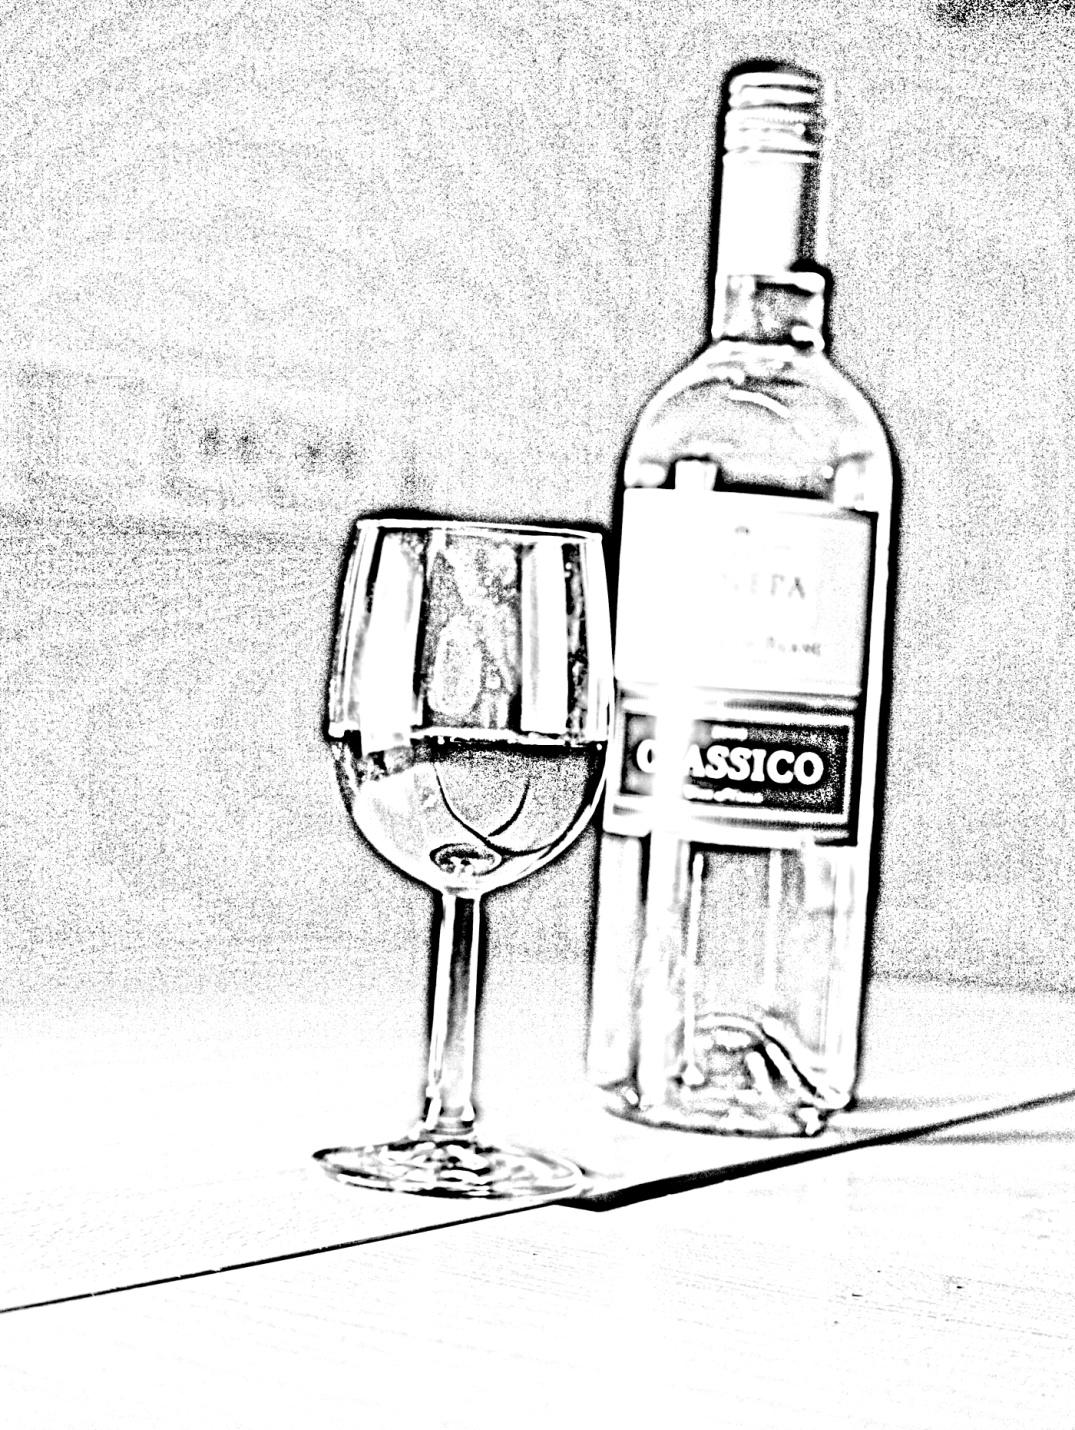
\includegraphics[width=0.8\textwidth]{res/vinvisor.jpg}
   \section{Vinvisor}
   
\end{center}
\vfill
\newpage


\subsection{Bordeaux, Bordeaux}
\textit{Mel: I sommarens soliga dagar}\\
\index[alfa]{Bordeaux, Bordeaux}
\index[anfa]{Jag minns än idag hur min fader...}
\begin{parse lines}[\noindent]{#1\\}

Jag minns än idag hur min fader
kom hem ifrån staden så glader
och rada upp flaskor i rader
och sade nöjd som så:
"Bordeaux, Bordeaux!"

Han drack ett glas, kom i extas,
och sedan blev det stort kalas.
Och vi små glin, ja vi drack vin
som första klassens fyllesvin.
Och vi dansade runt där på borden
och skrek så vi blev blå:
"Bordeaux, Bordeaux!”
\end{parse lines}


\subsection{Ismaskinen}
\textit{Mel: Nu så kommer julen, ur Karl-Bertil Johnssons julafton}\\
\textit{Lundakarnevalen 2002}\\
\index[alfa]{Ismaskinen}
\index[anfa]{Läpparna blir lila...}
\begin{parse lines}[\noindent]{#1\\}

Läpparna blir lila
när man dricker vin,
och om man har huvet
i en ismaskin!
\end{parse lines}


\subsection{Feta fransyskor}
\textit{Mel: Militärmarsch av Schubert}\\
\textit{K-sektionen Sångarstriden 1985}\\
\index[alfa]{Feta fransyskor}
\index[anfa]{Feta fransyskor som svettas om fötterna...}
\begin{parse lines}[\noindent]{#1\\}

Feta fransyskor som svettas om fötterna,
de trampar druvor
som sedan ska jäsas till vin.
Transpirationen viktig é,
ty den ge
fin bouquet.
Vårtor och svampar följer me
men vad gör väl de?

För vi vill ha vin,
vill ha vin,
vill ha mera vin,
även om följderna blir
att vi må lida pin.
Flaskan och glaset gått i sin.
Hit med vin, mera vin!
Tror ni att vi är fyllesvin?
Ja! Fast större!
\end{parse lines}
\vfill
\noindent\textit{Att man i slutet sjunger ”Ja! Fast större!” var inte menat från början, utan det var menat att tryckeriet skulle trycka ”Ja!” med större bokstäver.}



\subsection{Korkskruvens visa}
\textit{Mel: Nu har vi ljus}\\
\index[alfa]{Korkskruvens visa}
\index[anfa]{Nu har vi rus här i vårt hus...}
\begin{parse lines}[\noindent]{#1\\}

Nu har vi rus här i vårt hus
Korken är borta hopptralalala
Doften är ljuv, jag är en skruv,
jag är en skruv.

Jag kan inte öppna bag-in-boxen,
jag kan inte öppna bag-in-boxen

Lalalala lalalala lalalalala lala
\end{parse lines}


\subsection{Vinvännernas visa}
\textit{Mel: Imse vimse spindel}\\
\index[alfa]{Vinvännernas visa}
\index[anfa]{Åsnan dricker vatten, det gör inte vi...}
\begin{parse lines}[\noindent]{#1\\}

Åsnan dricker vatten, det gör inte vi.
Vi dricker bara sådant folk har trampat i.
Kamelen uti öknen söker en oas,
det gör inte vi, vi har vin i våra glas.

Imse vimse blir jag utav lite vin.
Kliver upp på stolen, och blir piggelin.
Trillar under bordet, sussar en minut.
Vaknar av att vinet nästan tagit slut.
\end{parse lines}


\subsection{Magnumflaskan Åkesson}
\textit{Mel: Teddybjörnen Fredriksson}\\
\index[alfa]{Magnumflaskan Åkesson}
\index[anfa]{För längesen, när jag fyllde 15 år...}
\begin{parse lines}[\noindent]{#1\\}

För längesen, när jag fyllde 15 år
fick jag en flaska av min mor.
Hon sa "Mitt barn, dela den med vännerna.
För den är faktiskt ganska stor."

Magnumflaskan Åkesson,
du var så stor och tung. 
Jag gick runt med dig i hand,
och i Dalby var jag kung.

Magnumflaskan Åkesson, 
din kork försvann i skyn.
Men jag drack dig bara själv.
Och kräktes i hela byn.
\end{parse lines}

\newpage
\subsection{Sprittillverkarvisan}
\textit{Mel: Mössens julafton}\\
\index[alfa]{Sprittillverkarvisan}
\index[anfa]{För väldigt många år sen plantera man i rad...}
\begin{parse lines}[\noindent]{#1\\}

För väldigt många år sen plantera man i rad
små rankor för att göra drycker så att man blev glad.
En druva skulle odlas och efter något år
bli plockad, trampad, tappad och sen fin Bordeaux.
Konstiga processer tog sin fart,
men det tog alltför många år för vinet att bli klart.
Ty idag med socker, jäst och vann
på någon dag man gör sin alkohol i spann.
\end{parse lines}

\newpage
\thispagestyle{empty}
\null
\vfill
\begin{center}
   
   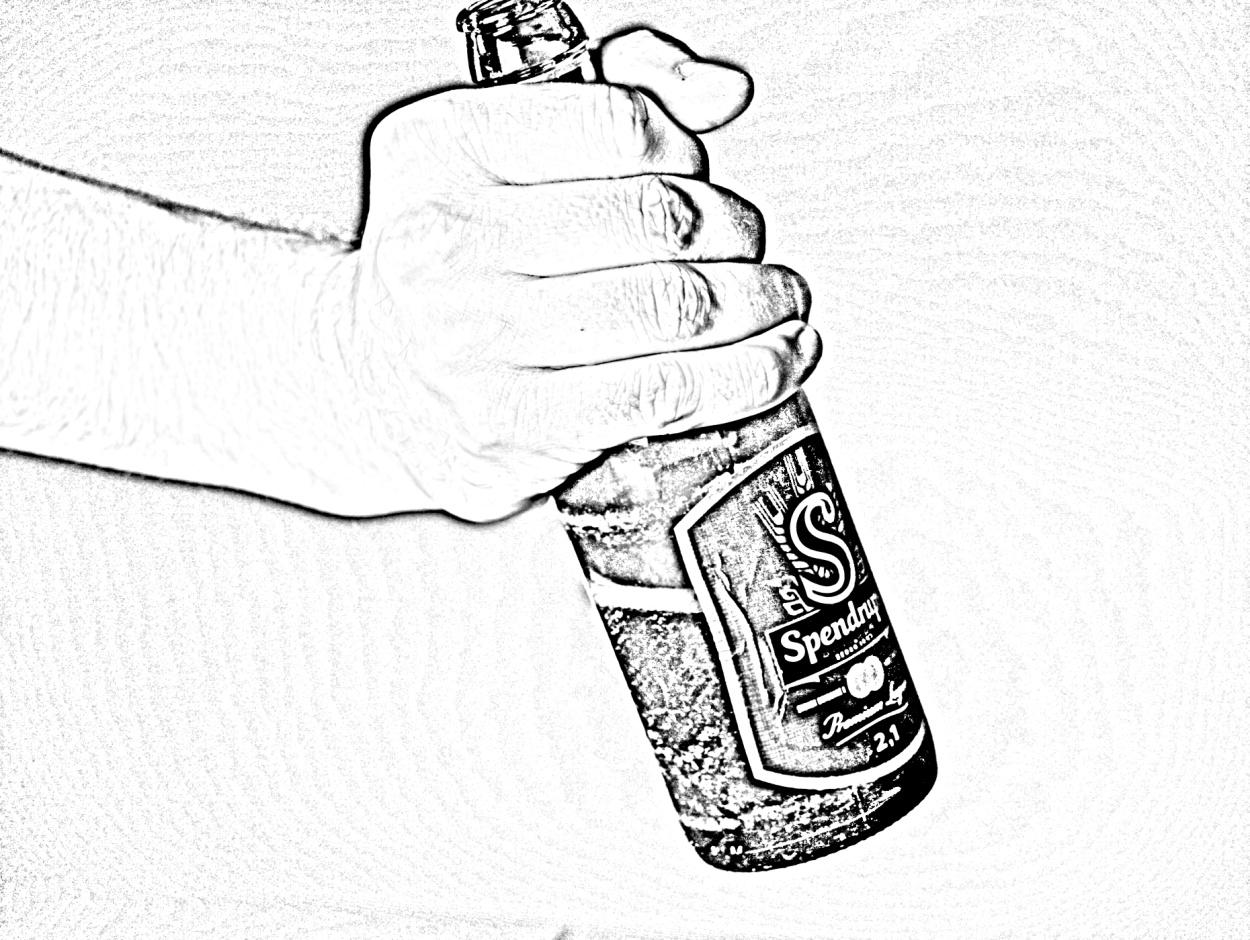
\includegraphics[width=1.0\textwidth]{res/olvisor.jpg}
   \section{Ölvisor}
   
\end{center}
\vfill
\newpage


\subsection{Hästhandlarn}
\textit{Mel: I ett hus vid skogens slut}\\
\textit{Vinnande ölvisa, Lundakarnevalen 1994}\\
\index[alfa]{Hästhandlarn}
\index[anfa]{Ur ett glas vid bordets slut...}
\begin{parse lines}[\noindent]{#1\\}

Ur ett glas vid bordets slut
liten starköl rinner ut
Lennart stirrar på sitt stop
bryter nog ihop
Nej, han vaknar ur sin nöd
cyklar hem till Veberöd
pantsätter sin systers föl
tusen spänn till öl
\end{parse lines}


\subsection{Öl!}
\textit{Mel: Var nöjd med allt som livet ger}\\
\index[alfa]{Öl"!}
\index[anfa]{Jag gillar alla sorters öl...}
\begin{parse lines}[\noindent]{#1\\}

Jag gillar alla sorters öl,
jag dricker dem med glädjebröl,
till frukost, lunch och middag varje dag!
Jag gillar öl för vet du vad?
Av bordsvatten blir ingen glad.
Nej, öl för fulla muggar vill jag ha.
\end{parse lines}

\newpage
\subsection{Strejk på Pripps}
\textit{Mel: I natt jag drömde}\\
\index[alfa]{Strejk på Pripps}
\index[anfa]{Inatt jag drömde något som...}
\begin{parse lines}[\noindent]{#1\\}

Inatt jag drömde något som,
jag aldrig drömt förut
Jag drömde det var strejk på Pripps 
och alla ölen var slut.
Jag drömde om en jättesal 
där ölen stod på rad
Jag drack sådär en femton 
öl och reste mig och sa:
"Man kan ha roligt utan sprit, 
men det är dumt att chansa."
\end{parse lines}

\vspace{-0.2cm}
\subsection{Vi älskar öl}
\textit{Mel: Ser du stjärnan i det blå}\\
\index[alfa]{Vi älskar öl}
\index[anfa]{Täckt av silver sejdeln full...}
\begin{parse lines}[\noindent]{#1\\}

Täckt av silver sejdeln full
gnistrar mot oss med sitt guld
humle, malt, är livets salt, vi älskar öl.

Källarsval så bärs den in
för att glädja gommen din
släcka törsten, stärka rösten, till dess lov.

Knubbig blir du, men so what
gott och roligt har du fått
extra turen, rensat njuren, öl är gott.
\end{parse lines}

\vspace{-1cm}
\subsection{Öl-kanon}
\textit{Mel: Row, row, row your boat}\\
\index[alfa]{Öl-kanon}
\index[anfa]{Drick, drick, drick din öl...}
\begin{parse lines}[\noindent]{#1\\}

Drick, drick, drick din öl
låt den rinna ner.
Kan du sen kraxa
"en laxask med slasktratt"
så får du dricka fler.
\end{parse lines}


\subsection{Ont i Huvudet}
\textit{Mel: Ingeborg}\\
\index[alfa]{Ont i Huvudet}
\index[anfa]{Om du har ont i huvet...}
\begin{parse lines}[\noindent]{#1\\}

Om du har ont i huvet
när du vaknar någon da
så häll en öl i håret
och låt den stå och dra.

Och känns det inte bättre
så skyll inte på oss,
Att hälla öl i huvet
är inte smart förstås.
\end{parse lines}


\vfill
\subsection{Ode till ölet}
\textit{Mel: Trampa på gasen}\\
\index[alfa]{Ode till ölet}
\index[anfa]{Tu tu tu Tuborg...}
\begin{parse lines}[\noindent]{#1\\}

Tu tu tu Tuborg
och ca ca ca Carlsberg
det är den bästa
pi pi pi pilsnern som jag vet

Tu tu tu Carlsberg
och ca ca ca Tuborg
det är det bästa
pi pi pi ölet som jag vet

Tu tu tu Ölberg
och ca ca ca Pilsborg
det är den bästa
pi pi pi biran som jag vet

Tu ca pi Ölsner
och pi tu ca bira
det är den bästa
ca pi tu lering som jag gjort
\end{parse lines}




\vfill
\subsection{Om en söt dryck}
\textit{Mel: En tokig sång}\\
\index[alfa]{Om en söt dryck}
\index[anfa]{Jag dricker gärna öl och vin...}
\begin{parse lines}[\noindent]{#1\\}

Jag dricker gärna öl och vin
till sillen tar jag nubben
och kanske till och med en shot
när jag har gått till klubben.

Men drycken som jag helst vill ha
den har så friska lukter
den är dessutom ren och klar
och smakar utav frukter

Hå hum, man é ej dum
för att man dricker cider
Även om, det finnes dom
som utav smaken lider

Det skummar upp i glaset när
man har hällt upp en cider
det smakar både sött och gott
när den i halsen glider

Det kan vá både söt och torr
av tranbär eller fläder
av plommon och det finns nån sort
som smakar gamla kläder

Hå hum, man é ej dum...
\end{parse lines}

\vspace{-0.9cm}
\subsection{Ölets kretslopp}
\textit{Mel: Auld Lang Syne}\\
\textit{Vinnande bidrag bordsvisesittning 2018}\\
\index[alfa]{Ölets kretslopp}
\index[anfa]{Om någon gång du spillt din öl...}
\begin{parse lines}[\noindent]{#1\\}

Om någon gång du spillt din öl
Och gråtit över det
Om någon gång du spillt din öl
Då hoppas jag du vet

Att vattnet har ett kretslopp som
För ölen upp i sky
$\vert\vert$: Så nästa gång som regnet kom
Bli full på homeopati :$\vert\vert$
\end{parse lines}
\vfill
\noindent\textit{De sista två raderna kan sjungas X antal gånger där $2\leq$ X $\leq$ $ \sim33$.}

\newpage
\subsection{Udflykt til Danmark}
\textit{Mel: Mitt lilla fejs och jag}\\
\textit{K-sektionen Sångarstriden 1992}\\
\index[alfa]{Udflykt til Danmark}
\index[anfa]{Om du har det trist i Lund...}
\begin{parse lines}[\noindent]{#1\\}

Om du har det trist i Lund,
åk över Öresund.
Sätt dig på en färja,
sen så kan du härja.
Köp en öl, köp en till
eller Köpenhamn
köp så mycket öl du vill,
smuggla om du kan.

Man kan se på konst, jovisst,
på Louisiana
men visst är det ganska trist,
bara gå och glana.
Så vi kör till Helsingör,
köper lite smör.
Heja Danmark friskt humör,
sjunger vi i kör.

Många søde piger finns,
dejligt sensuella
men man bör se upp med kvinns,
tänk på salmonella.
Lajbans hela natten lång,
festa som en vilde.
Rockmusik och hålligång,
värre än Roskilde.

Nästa morgon, nästan död,
står man där i tullen.
Näsan lyser vit och röd,
halsen den är svullen.
Jag ska smuggla kött och öl,
men vad smugglar du?
Och du svarar med ett bröl:
"Den lille havefrue!
\end{parse lines}


\subsection{Prostatabesvär}
\textit{Mel: I Apladalen i Värnamo}\\
\index[alfa]{Prostatabesvär}
\index[anfa]{Jag kissar inte nån fin parabel...}
\begin{parse lines}[\noindent]{#1\\}

Jag kissar inte nån fin parabel.
Jag har fått nått hinder uti min snabel.
Ja, dricka öl ställer till besvär,
med en prostata som denna här.
\end{parse lines}


\newpage

\subsection{Ölen är slut}
\textit{Mel: Havet är djupt}\\
\index[alfa]{Ölen är slut}
\index[anfa]{Det börjar bli sent på festen...}
\begin{parse lines}[\noindent]{#1\\}

Det börjar bli sent på festen
och alla har jävligt kul.
Du slog din rival på beerpong
och din dans börjar bli ful.

Men du kan ej begripa
rösten som kallar ut.
"Det där var vår sista IPA
och nu så är ölen slut!"
Åh nej!

Ölen är slut!
Ölen är slut!
Ända till Lomma,
är burkarna tomma.
Ölen är slut!
I kylskåpet finns ju ingenting,
förutom tacos och powerking.
Så om du vill halsa,
nöj dig med salsa.
Ölen är slut!

Hos grannen är alla glada,
dit floder av IPA når,
men här på efterfesten
rinner endast en tår.
Du mister ditt lugn i krisen
och slutar att vara snäll.
Sen cakear du på polisen
och hamnar i fyllecell.
Åh nej!

Ölen är slut!
Ölen är slut!
Så drick mer vatten,
sov gott om natten,
sen pustar vi ut.
I kylskåpet finns ju ingenting,
förutom tacos och powerking.
Så om du vill halsa,
nöj dig med salsa.
Ölen är slut!
\end{parse lines}
\newpage
\null

\newpage
\thispagestyle{empty}
\null
\vfill
\begin{center}
   
   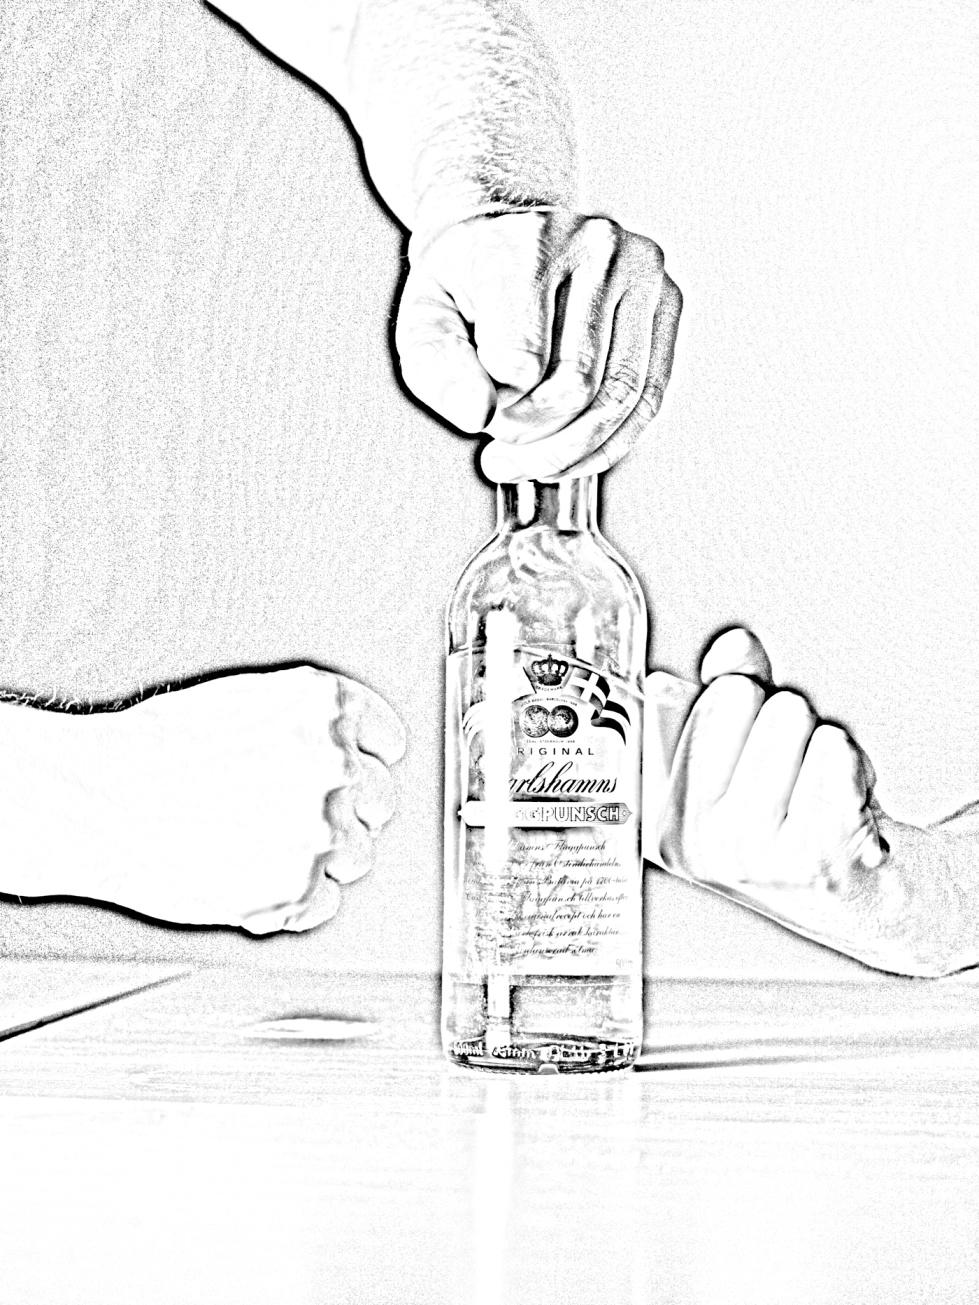
\includegraphics[width=0.9\textwidth]{res/punschvisor.jpg}
   \section{Punschvisor}
   
\end{center}
\vfill
\newpage

\subsection{Punschen kommer (kall)}
\textit{Mel: Vals ur Glada Änkan}\\
\index[alfa]{Punschen kommer (kall)}
\index[anfa]{Punschen kommer, punschen kommer...}
\begin{parse lines}[\noindent]{#1\\}

Punschen kommer, punschen kommer,
ljuv och sval.
Glasen imma, röster stimma
i vår sal.
Skål för glada minnen!
Skål för varje vår!
Inga sorger finnas mer
när punsch vi får.
\end{parse lines}


\subsection{Punschen kommer (varm)}
\textit{Mel: Vals ur Glada Änkan}\\
\index[alfa]{Punschen kommer (varm)}
\index[anfa]{Punschen kommer, punschen kommer...}
\begin{parse lines}[\noindent]{#1\\}

Punschen kommer, punschen kommer,
god och varm.
Vettet svinner, droppen rinner
ner i tarm.
Skål för glada minnen!
Dem vi snart ej ha,
då ett par glas simmig punsch
vi hunnit ta.
\end{parse lines}

\newpage
%
\includegraphics[height=0.2\textheight]{res/kretslopp.png} 
%\vspace*{-0.2\textheight}

\begin{picture}(50,50) \put(155,0){\hbox{
\includegraphics[height=0.15\textheight]{res/kretslopp.png}}} \end{picture}
\vspace*{-0.20\textheight}


\subsection{Kretsloppet}
\textit{Mel: Nu har vi ljus}\\
\index[alfa]{Kretsloppet}
\index[anfa]{Genom vår kropp, ända till snopp...}
\begin{parse lines}[\noindent]{#1\\}

Genom vår kropp, ända till snopp,
punsch håller färgen, hopp, tralalala.
Kolla ditt kiss, ser du, jovisst, ser du, jovisst!
Samma gyllengula ädla vätska,
samma dryck som nyss vår tunga läska
tralalala lalalalala lalalalala lalala.

Tar punschen slut, spar på ditt krut,
skjut inte värden, hopp, tralalala.
Låt punschen gå varv nummer två, varv nummer två:
Två och två ni mot varandra ilar,
snart i munnen punschen åter strilar
tralalala lalalalala lalalalala lalala.
\end{parse lines}


\subsection{Gula droppar}
\textit{Mel: Midnatt råder}\\
\index[alfa]{Gula droppar}
\index[anfa]{Punschen, punschen rinner genom strupen...}
\begin{parse lines}[\noindent]{#1\\}

Punschen, punschen rinner genom strupen,
ner i djupen.
Blandas, konfronteras där med supen,
där med supen.
Gula droppar stärker våra kroppar,
PUNSCH, PUNSCH, PUNSCH!
\end{parse lines}



\subsection{Punschens lov}
\textit{Mel: Rövarna från Kamomilla stad}\\
\index[alfa]{Punschens lov}
\index[anfa]{Ja, punschen är och punschen var...}
\begin{parse lines}[\noindent]{#1\\}

Ja, punschen är och punschen var
och punschen skall förbliva.
En lidelse vi alla har
som inget kan fördriva.
Ja, punschen tinar opp, såväl
som svalkar både kropp och själ.
Den botar begären och lindrar besvären.
Ja, punschen den gör både gott och väl!
\end{parse lines}


\subsection{När kaffet är serverat}
\textit{Mel: Mössens julafton}\\
\textit{Sångarstriden 1987}\\
\index[alfa]{När kaffet är serverat}
\index[anfa]{När kaffet är serverat, och maten tagit slut...}
\begin{parse lines}[\noindent]{#1\\}

När kaffet är serverat, och maten tagit slut,
och alla dom som blivit alltför fulla kastats ut,
då vill vi ha ett nytt glas med något gult och kallt
som höjer och förbättrar vår promillehalt:
Arrak, etanol och sackaros med salt och vatten blir
den bästa blandning som kan fås.
Söt och smetig, rent utav viskös.
En sexton, sjutton glas så blir du medvetslös.
\end{parse lines}


\subsection{Anti-atkinsmetoden}
\textit{Mel: My darling Clementine}\\
\index[alfa]{Anti-atkinsmetoden}
\index[anfa]{Äter bara proteiner...}
\begin{parse lines}[\noindent]{#1\\}

Äter bara proteiner,
till min frukost och till lunch.
GI-kost och vitaminer,
tills det blivit dags för punsch.

Sedan blir det för besvärligt,
punschen är ju obligat.
Det är alltid lika härligt,
att bli full på kolhydrat.
\end{parse lines}

\newpage
\null
\newpage
\thispagestyle{empty}
\null
\vfill
\begin{center}
   
   
\includegraphics[width=0.9\textwidth]{res/hyllningsvisor.jpg}
   \section{Hedrande visor}
   
\end{center}
\vfill
\newpage

\subsection{Hyllningssång till D-sektionen}
\textit{Mel: Rövarna från Kamomilla stad}\\
\index[alfa]{Hyllningssång till D-sektionen}
\index[anfa]{Det hände nånting -82...}
\begin{parse lines}[\noindent]{#1\\}

Det hände nånting -82
ett minne värt att plockas.
När axelvaddar ej var små
och håret skulle lockas.
Från LTH ett glädjetjut
en sen augustidag steg ut, när
Åström, Arosenius, Blomquist, Johannesson
startat en Datatekniksektion.

Vår studierektor Wittenmark
ett liv för D fick blåsa.
Ett märke värdigt vår monark
vi fick i färgen råsa.
Studenterna blev glada för
ett byte från en brun kulör.
Med 15 mot 14 i skär attraktion.
Resultatet: en råsa ny D-sektion.

Det gick ett år, sen gick det tre,
sektionen börja blomma.
Man startade ett D-café
och cyklade till Lomma.
Med Nollningar som inte fanns
blev D-sek en speciell instans,
där saker blev gjorda av ren affektion
till vår kära, uppskattade D-sektion.

Nu fyrtio år D funnits har,
vi firar det med fester.
Vi stöter ut en stor fanfar
med hjälp av vår orkester.
Vi hoppas att om fyrtio år
man sitter här som senior.
Och lyssnar på någon med samma passion
såsom vi har för vår kära D-sektion.
\end{parse lines}

\noindent\textit{Skrevs till 20-års jubileumet, men sista versen skrevs om till 30-års jubileumet, och sedemera även till 40-årsjubileumet:
} 

\noindent\textit{preg\_replace(”tjugo”, ”trettio”, \$sang);
}

\noindent\textit{preg\_replace(”trettio”, ”fyrtio”, \$sang);
}






\subsection{Data, data, ingen slår ju Data}
\textit{Mel: Bamse}\\
\index[alfa]{Data, data, ingen slår ju Data}
\index[anfa]{Data, data, ingen slår ju data...}
\begin{parse lines}[\noindent]{#1\\}

Data, data, ingen slår ju data
För vi tycker inte om att slåss
Kramas gör vi för att inte hata
Därför är ju segern vår förstås

Data, data, data, ...  ...InfoCom
\end{parse lines}


\newpage
\subsection{D-sek, D-sek}
(Ramsa)\\
\begin{parse lines}[\noindent]{#1\\}

Dsek, dsek, vi går på dsek
Kompilera källkod så får du exe

Exe, exe,
Går det med java?
Går det?
Jaaarrr
\end{parse lines}



\subsection{Störst o bäst!}
\textit{Mel: Who’s that lying on the runway? }\\
\index[alfa]{Störst o bäst"!}
\index[anfa]{Vem e’ störst o bäst i Skåne?}
\begin{parse lines}[\noindent]{#1\\}

Vem e’ störst o bäst i Skåne? 
Vem e’ kung på LTH? ”ja LTH”
Ja de’ e’ Data-InfoCom
Som hela festen drar igång
Tacka Gud för Data-InfoCom
\end{parse lines}

\newpage
\subsection{Källarsektionen}
\textit{Mel: Rule Britannia}\\
\textit{Skriven av Oskar Ström}\\
\index[alfa]{Källarsektionen}
\index[anfa]{D-sektionen, vi gömmer oss för solen...}
\begin{parse lines}[\noindent]{#1\\}

D-sektionen 
Vi gömmer oss för solen
D-sek har källarfest 
Ja D-sek är bäst
\end{parse lines}

\subsection{Skär och gredelin}
\textit{Mel: Oh, when the saints}\\
\textit{Nollespexet F-sektionen 2007}\\
\index[alfa]{Skär och gredelin}
\index[anfa]{Jag vill va skär...}
\begin{parse lines}[\noindent]{#1\\}

Jag vill va skär
och gredelin!
Det får man inte på maskin!
Där ska man dricka stora mängder alkohol
och vara jävligt maskulin!
\end{parse lines}

\newpage
\subsection{Man ska gå Data!}
\textit{Mel: Man ska ha husvagn}\\
\index[alfa]{Man ska gå Data"!}
\index[anfa]{Ni har pluggat nästan allt som går att plugga på...}
\begin{parse lines}[\noindent]{#1\\}

Ni har pluggat nästan allt som går att plugga på.
Räknat matte, läst kemi och lärt er flera språk.
Efter alla dessa år är valet väldigt lätt,
För er vill vi berätta att valet ert är rätt.

Man skall gå Data!
Då vet man ett plus ett är noll
Man skall gå Data
Det gör ju alla som har koll
Man skall gå Data
Det vill ju varje ingenjör
Man skall gå Data
Som sig alla bör
Men än så länge är ni allihopa bara nollor
För att lyckas bli en etta krävs det mer än bara fyllor.
En Dataingenjör den orkar både natt som dag.
Fixar plugget, klarar festen, gillar hårda tag!

Man skall gå…Fem minuter Java, C. Fem minuter Unix.
Fem minuter groggbuffé. Fem minuter drinkmix.
Fem minuter tentaplugg. Fem minuter gasque.
Fem minuter efter tentan blir det ET-slasque.

Man skall gå…
\end{parse lines}





\subsection{Datatekniksektionens sommarvisa}
\textit{Mel: Idas sommarvisa}\\
\index[alfa]{Datatekniksektionens sommarvisa}
\index[anfa]{I Sverige finns det många högskolor...}
\begin{parse lines}[\noindent]{#1\\}

I Sverige finns det många högskolor
där ungdomar utbildning får
vid högskolorna finns sektionerna
med det finns en sektion ingen slår.

Den bästa av alla sektionerna
är Data-sektionen såklart.
Här frodas vi råsa och lyckliga
och livet är helt underbart.

Vi leker försiktigt i gröngräset
och solar oss på sjön Sjøns strand
vi kramas med alla vi träffar på
och håller varandra i hand.
\end{parse lines}


\subsection{D-soldat}
\textit{Mel: Jag är en astronaut}\\
\index[alfa]{D-soldat}
\index[anfa]{Jag är en D-Soldat...}
\begin{parse lines}[\noindent]{#1\\}

Jag är en D-Soldat.
Jag är en D-Soldat.
K:are, F:are, Eko, E,
Dom slänger jag i spat.
\end{parse lines}

\subsection{C is for cookie}
\textit{Mel: C is for cookie}\\
\textit{InfoCom:s officiella visa}\\
\index[alfa]{C is for cookie}
\index[anfa]{Now what starts with the letter C..?}
\begin{parse lines}[\noindent]{#1\\}

(talat)
Now what starts with the letter C..?
Cookie starts with C!
Let's think of other things that starts with C...
Ah, who cares about other things?!

(sång)
$\vert\vert$: C is for cookie, that's good enough for me
C is for cookie, that's good enough for me
C is for cookie, that's good enough for me, ooh
Cookie, cookie, cookie starts with C :$\vert\vert$

(talat)
Hey, you know what?
A round cookie with one bite out of it looks like a C.
A round doughnut with one bite out of it also looks like a C,
but it is not as good as the cookie!
The moon sometimes looks like a C, but you can't eat that, so...

(sång)
C is for cookie, that's good enough for me
C is for cookie, that's good enough for me
C is for cookie, that's good enough for me, ooh
Cookie, cookie, cookie starts with C, yeah!
Cookie, cookie, cookie starts with C, oh boy!
Cookie, cookie, cookie starts with C!
\end{parse lines}


\subsection{Diskho-tankar}
\textit{Mel: My darling Clementine}\\
\index[alfa]{Diskho-tankar}
\index[anfa]{Jag diskar knivar...}
\begin{parse lines}[\noindent]{#1\\}

Jag diskar knivar,
jag diskar gafflar,
jag diskar skedar,
jag diskar disk.
Jag diskar muggar,
jag diskar tallrik.
Jag rensar formar
från gammal fisk.

Jag följer Star Trek,
jag spelar rollspel,
jag äter pizza,
jag kodar C.
Mitt liv är stressigt,
jag kuggar tentor.
Min själ är rosa,
jag  läser D! 
\end{parse lines}


\newpage
\null
\newpage
\thispagestyle{empty}
\null
\vfill
\begin{center}
   
   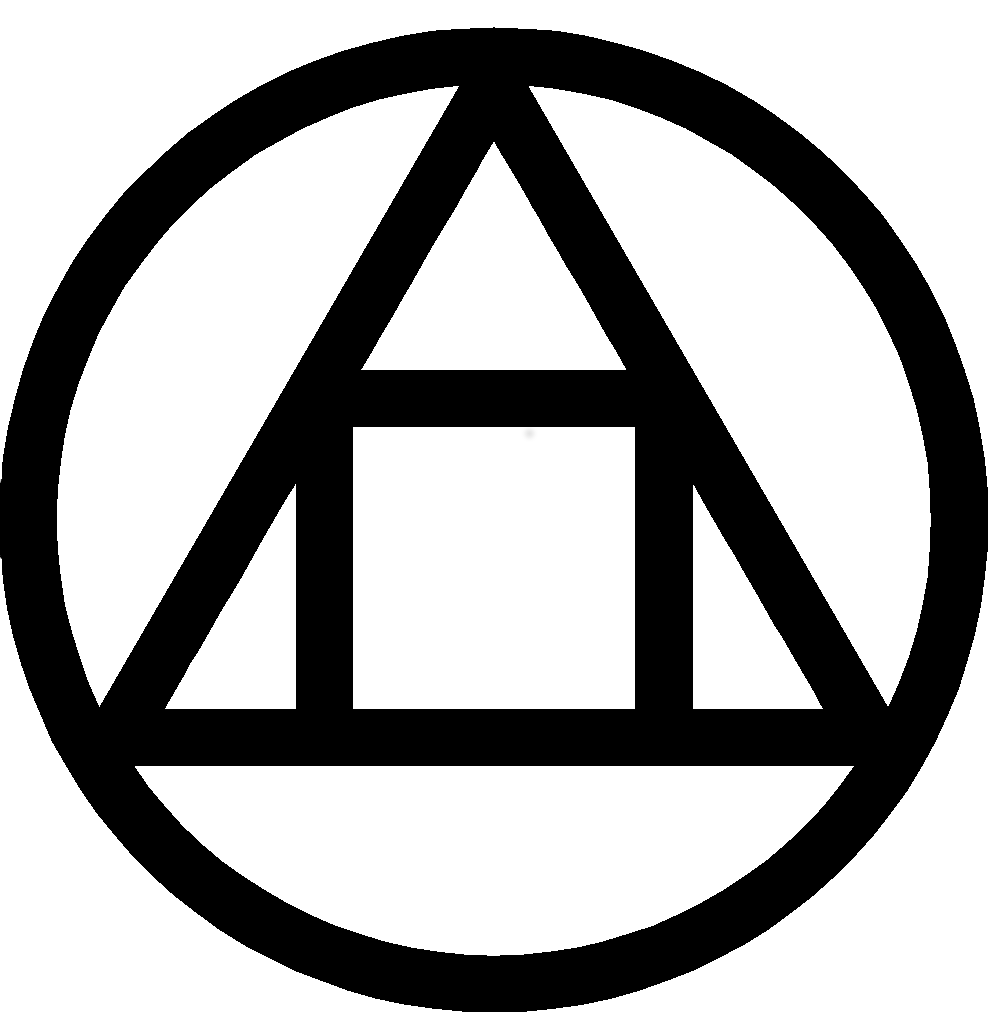
\includegraphics[width=0.9\textwidth]{res/sektionsvisor.png}
   \section{Sektionsvisor}
   
\end{center}
\vfill
\newpage

\subsection{Hyllningsvisa till Teknisk Fysik}
\textit{Mel: Sit on my face}\\
\index[alfa]{Hyllningsvisa till Teknisk Fysik}
\index[anfa]{Teknisk Fysik är mössbeklädda töntar...}
\begin{parse lines}[\noindent]{#1\\}

Teknisk Fysik är mössbeklädda töntar
fula flickor och en samling mammas pojkar.
Liknar mest en televerksbil, 
som gått för många mil
En teknisk fossil!

Teknisk Fysik är lättare än att fjärta
Döda älgar värmer nu mitt kalla hjärta
Ta hit dynamit, sprängteknik, vårt gebit
Dessa tofsprydda avskum som ger oss kolik!
Dessa tofsprydda avskum som ger oss kolik!
Dessa tofsprydda avskum som ger oss kolik!
Dessa tekniska lik! Barambam!
\end{parse lines}
\vfill
\textit{Skrevs av V-sektionen till en Sångarstrid, men stals lumpet av F-sektionen som framförde den innan V fick chansen.}

\subsection{Everywhere we go}
\textit{Mel: Everywhere we go}\\
\index[alfa]{Everywhere we go}
\index[anfa]{Everywhere we go...}
\begin{parse lines}[\noindent]{#1\\}

Everywhere we go
People wanna know
Who we are
So we tell them

We are the E-sek
Mighty, mighty E-sek

$\vert\vert$: Uh, ah, oh E-sek :$\vert\vert$ (3 ggr)
\end{parse lines}

\subsection{Vår färg är röd}
\textit{Mel: When the saints go marching in}\\
\index[alfa]{Vår färg är röd}
\index[anfa]{Vår färg är röd}
\begin{parse lines}[\noindent]{#1\\}

Vår färg är röd, vår färg är fin,
för det är vi som går Maskin
Och vi har kommit för att dricka alkohol,
för det är vi som går Maskin
\end{parse lines}

\newpage
\subsection{Brand, Lant, Väg och Vatten}
\textit{Mel: Högst vinner}\\
\index[alfa]{Brand, Lant, Väg och Vatten}
\index[anfa]{Brand, Lant, Väg och Vatten...}
\begin{parse lines}[\noindent]{#1\\}

Brand, Lant, Väg och Vatten,
Störst på LTH
Ingenting kan stoppa oss,
V-sek allez allez 
\end{parse lines}


\subsection{A-sek är bäst}
\textit{Mel: Rule Britannia}\\
\index[alfa]{A-sek är bäst}
\index[anfa]{A-sektionen den skiner såsom solen...}
\begin{parse lines}[\noindent]{#1\\}

A-sektionen den skiner såsom solen.
A-sek är grym på fest, ja A-sek är bäst!
\end{parse lines}



\newpage
\subsection{Kemisternas kampvisa}
\textit{Mel: Eslövs nationalsång}\\
\index[alfa]{Kemisternas kampvisa}
\index[anfa]{Vi är kemister och vi älskar maskinister...}
\begin{parse lines}[\noindent]{#1\\}

Vi är kemister och vi älskar maskinister
Vi är kemister och vi pussar arkitekt
Vi är kemister och vi kramar väg och vatten
Vi är kemister och vi är allra bäst!

Å.. spela, spela data!
Å.. heja, heja F!
Å.. koppla in elektro!
Å.. men K är allra bäst!
\end{parse lines}


\subsection{ING från sundets pärla}
\textit{Mel: Whistle stop (från Robin Hood)}\\
\index[alfa]{ING från sundets pärla}
\index[anfa]{För vi är ING från sundets pärla...}
\begin{parse lines}[\noindent]{#1\\}

För vi är ING från sundets pärla,
och det är fest idag igen,
och vi ska supa hela natten lång 
och sjunga denna sång!

Raj-di-daj-daj-daj…
\end{parse lines}

\newpage
\subsection{Turkosa samban}
\textit{Mel: Samba de Janeriro }\\
\index[alfa]{Turkosa samban}
\index[anfa]{SAMBA"! Turkos turkos, här gör vi entré...}
\begin{parse lines}[\noindent]{#1\\}

SAMBA!

Turkos turkos, här gör vi entré
Vi bränner sprit uti KC:G
Turkos turkos, så gör dubbel-W
Mitt glas är två för att jag är sne!

$\vert\vert$: Simma sí, ah simma, 
ah simma simma simma :$\vert\vert$ (4ggr)
\end{parse lines}


\subsection{Bortom vägar och vatten}
\textit{Mel: Pomp and Circumstance}\\
\index[alfa]{Bortom vägar och vatten}
\index[anfa]{Bortom vägar och vatten...}
\begin{parse lines}[\noindent]{#1\\}

Bortom vägar och vatten, 
långt långt över Maskin
innan Brand hunnit släckas, 
blickar vi ner på Kemi.
Bam bam bam!
Stolta står vi och väntar, 
tills Elektro gjort sin sorti,
för vi är bästa sektionen, 
och vi älskar vårat I!
\end{parse lines}

\newpage
\thispagestyle{empty}
\null
\vfill
\begin{center}
   
   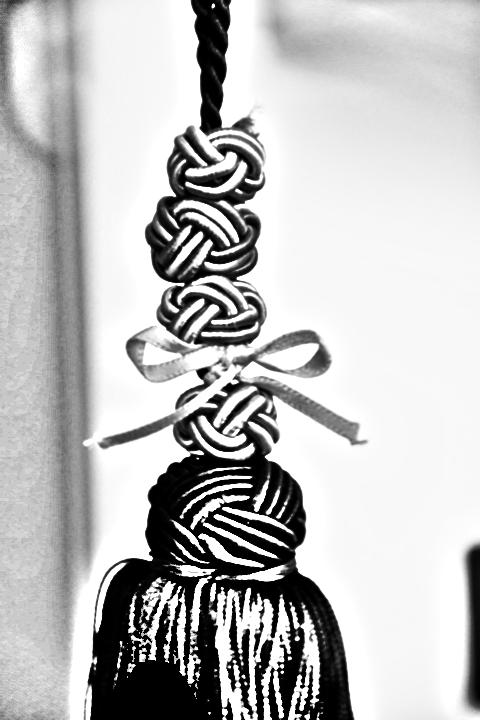
\includegraphics[width=0.8\textwidth]{res/dchip.jpg}
   \section{D-Chip}
   
\end{center}
\vfill
\newpage



\subsection{D-Chip är grymt}
\textit{Mel: Havet är djupt}\\
\index[alfa]{D-Chip är grymt}
\index[anfa]{De tror att det inte finns nå-...}
\begin{parse lines}[\noindent]{#1\\}

De tror att det inte finns nå-
gra tjejer på vår sektion.
Att vi bara dricker lättöl,
vad e det för slags fason?
Nej se dig omkring på dsek,
här finns vi och lustigt e
du kan inte bli besviken
det ska du snart få se!

att

D-Chip är grymt
D-Chip är grymt
Utanför källarn
är vi rätt sällan
men nu har vi rymt (alt. här får ni en skymt)

Å ganska råsa är vi här
så sjung nu så högt som rösten bär
för datatjejer 
här har ni grejer
D-Chip är grymt!
\end{parse lines}


\subsection{Vill du koda med mig?}
\textit{Mel: Om sanningen ska fram}\\
\index[alfa]{Vill du koda med mig?}
\index[anfa]{Om jag lär mig alla namnen...}
\begin{parse lines}[\noindent]{#1\\}

Om jag lär mig alla namnen,
och Spritbolagets svans,
Om jag lär mig nollevisan, 
skyddar chepsen med mitt liv.

Om jag köper mig en ouvve,
syr märken som en Gud.
Om jag respekterar staben,
lär mig våran nolledans.

$\vert\vert$: Vill du koda med mig då? Om sanningen ska fram?
Vill du koda med mig då? Vill du koda med mig? :$\vert\vert$ 

Om jag lär mig dricka minttu,
fast det faktiskt smakar skit.
Spöar phaddrarna på beer pong,
sätter trick shotsen från taket.

Och som alla phaddrar säger:
“Ingen hets, men det blir kul,
och det kommer säljas dricka
hashtag omduvill”

$\vert\vert$: Vill du koda med mig då? Om sanningen ska fram?
Vill du koda med mig då? Vill du koda med mig? :$\vert\vert$ 
\end{parse lines}
\subsection{Microchipvisa 2000}
\textit{Mel: Fångad av en stormvind}\\
\index[alfa]{Microchipvisa 2000}
\index[anfa]{Det folk inte kan förstå...}
\begin{parse lines}[\noindent]{#1\\}

Det folk inte kan förstå
Är kärleken som finns över Internet
Mina vänner undrar så
varför hjärtat bultar hårt när jag loggar in igen
Känslan när jag ser ditt namn på min skärm
pulsen ökar och jag blir alldeles varm

Jag är fångad med ett bredband, föll för dig,
när du skrev ett mejl till mig
du finns lagrad i mitt hjärta
Fångad med ett bredband, natt och dag
sitter jag här ensam kvar,
och väntar på din bild som laddas ner.

Jag borde ge mig av
för tiden går så fort i en datasal
Men min känsla stannar kvar
det är något som jag skulle ha förstått.
Jag vänder om igen och ser mig nu omkring
mejlen kommer ju från datorn bredvid mig.

Jag är fångad av en D-grabb, dig förstås.
Ingen alls kan hindra oss,
nu när skolan ligger öde.
Jag har fått en jackpot, här hos mig,
nu ska jag förföra dig,
i det ljus som skärmen strålar ut.

Vi surfar långsamt
uppkopplad på kärlekens band
Min längtan vaknar
när du ler
på väg mot cyberland
\end{parse lines}

\newpage
\null
\newpage
\thispagestyle{empty}
\null
\vfill
\begin{center}
   
   
\includegraphics[width=1.0\textwidth]{res/nordigavisor.jpg}
   \section{Nördiga visor}
   
\end{center}
\vfill
\newpage

\subsection{IQ-test}
\vfill
\begin{center}
   
   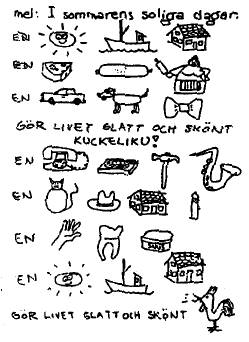
\includegraphics[width=1.0\textwidth]{res/iqtest.png}
   
\end{center}
\vfill
\newpage

\subsection{CVS-visan}
\textit{Mel: Odefinierad/Valfri}\\
\index[alfa]{CVS-visan}
\index[anfa]{Status told there's something new...}
\begin{parse lines}[\noindent]{#1\\}

Status told there's something new
UPDATE, UPDATE, UPDATE, COMMIT

Many files or just a few
UPDATE, UPDATE, UPDATE, COMMIT

We don't need to hope and pray
UPDATE, UPDATE, UPDATE, COMMIT

'cause we work the clever way
UPDATE, UPDATE, UPDATE, COMMIT
\end{parse lines}

\noindent\textit{(Rad i gemener sjunges av försångare)\\
Sjungs av Lars Bendix på någon föreläsning i kursen EDA260.}




\subsection{D-visor}
\textit{Mel: Row, row, row your boat}\\
\index[alfa]{D-visor}
\index[anfa]{$\rho\  \rho\  o...$}


\noindent $\rho\  \rho\  o \\
\lambda\  \sigma\  \xi \\
\nu\  \varepsilon\  \delta\  \mu\  \varphi \\
\theta\  \kappa\  \pi $\\


\subsection{En komplex värld}
\textit{Mel: En helt ny värld}\\
\index[alfa]{En komplex värld}
\index[anfa]{Alla jävla bevis...}
\begin{parse lines}[\noindent]{#1\\}

Alla jävla bevis
inses lätt som en övning.
Javakursen en prövning
för min bristande logik.

Ska man komma ihåg
alla formler i huvet?
Formelsamlingen, du vet,
säger inget om det här!

En komplex värld
Vad fan betyder bijektiv?
Ingenting stämmer här, där allt jag lär,
blir glömt snart efter tentan.
Hur ska det gå?
Och det är bara vecka två...
Känner en underton av aggression
mot allt Sven Spanne skrivit i sin bok

(Jag kan transponera den...)

Jag kan lära dig C
Matematiska under
Oförglömliga stunder
när vi tentar mekanik

Det ska nog gå!
Det sa din mamma med igår
All tid tillvaratas, jag är i fas,
och bor i mattehuset.
Nu är jag lärd!
Till denna svåra ekvation
jag på frekvenssidan en lösning fann,
den låg där i en helt ny värld: Laplace!
\end{parse lines}


\subsection{SI}
\textit{Mel: Studentsången}\\
\index[alfa]{SI}
\index[anfa]{W kg m Wb s...}

\noindent W kg m Wb s \\
$\Omega$ m T A rad \\
cd Sv N s \\
$\Omega$ A m lx dB \\
\degree C\  W/$m^{2}$ \\
J/kg\ H\ V\ C \\
kg/$m^{3}$ mol \\
m/$s^{2}$, m/$s^{2}$ \\
F!

\vfill
\subsection{Man ska ha MATLAB}
\textit{Mel: Man ska ha husvagn}\\
\vspace{-1.2cm}
\begin{parse lines}[\noindent]{#1\\}
\index[alfa]{Man ska ha MATLAB}
\index[anfa]{Jag har prövat nästan allt som finns att pröva...}\\

Jag har prövat nästan allt som finns att pröva på
Beta, kulram, räknesticka, tärning eller så
Jag har kalkylerat på de konstigaste sätt
och nu så har jag kommit på hur man ska räkna rätt

Man ska ha MATLAB -  då är kalkylen redan klar
Man ska ha MATLAB -  det har jag sett att andra har
Man ska ha MATLAB -  det är min livsfilosofi
Man ska ha MATLAB -  för då blir man fri

I många år så var jag inte alls så särskilt lärd
Jag visste ej vad som vänta mig i denna stora värld
Men sen kom jag till LTH, och ända sedan dess
så har jag funnit livets stora lyxdelikatess

Man ska ha MATLAB – så man slipper tänka alls
Man ska ha MATLAB -  ja, då går allting som en vals
Man ska ha MATLAB -  det bygger på nån slags logik
Man ska ha MATLAB - för då blir man rik

5 minuter mekanik och 5 minuter statfys
5 minuter plottande och 5 minuter analys
5 minuter fråga phadder, 5 minuter stopp
5 minuter tänka själv och sen så ger man opp

Man ska ha MATLAB - och datasalens friska luft
Man ska ha MATLAB - det tycker tjejerna är tufft
\makebox[\textwidth][s]{Man ska ha MATLAB - när ryssen kommer med sitt MIG}
Man ska ha MATLAB - då vinner man i krig!
\end{parse lines}\\
\textit{x = [-2:.001:2];}\\
\textit{y = real(($sqrt(cos(x)).*cos(200*x) $ $+$}\\
\textit{$sqrt(abs(x))-0.7).*(4-x.*x).\string^ 0.01);$}\\
\textit{plot(x,y);}




\subsection{Tänk om jag vore en liten kompilator}
\textit{Mel: Tänk om jag hade en liten liten apa}\\
\index[alfa]{Tänk om jag vore en liten kompilator}
\index[anfa]{Tänk om jag vore en liten kompilator...}
\begin{parse lines}[\noindent]{#1\\}

Tänk om jag vore en liten kompilator
Oompa oompa fallerallera,
Då skulle alla ha mig i sin dator,
Oompa oompa fallerallera

Tänk om jag vore ett Java Runtime Error
Oompa oompa fallerallera,
Då skulle alla drabbas av min terror
Oompa oompa fallerallera
\end{parse lines}

\vfill
\subsection{All you need is bredband}
\textit{Mel: John Brown’s body}\\
\index[alfa]{All you need is bredband}
\index[anfa]{Bredband, bredband, halleluja...}
\begin{parse lines}[\noindent]{#1\\}

$\vert\vert$: Bredband, bredband, halleluja :$\vert\vert$ (3ggr)
Bredband, bredband, bredband!

Suuurfa, surfa, surfa, surfa,
Surfa, surfa, surfa, surfa, suuurfa,
Surfa, surfa, surfa, surfa, surfa, surfa, surfa, surfa,
Det är det som är livets mening och mål!

Bredband! Bredband! Brrrrrrrredband!

$\vert\vert$: Bredband, bredband, halleluja :$\vert\vert$ (3ggr)
Bredband, bredband, bredband!

Innehållet, det kan kvitta!
Innehållet, det kan kvitta!
Porr och chatt, quake och tetris,
Klicka här för en bild på vår hund,
Det kräver två megabit per sekund!

Det ska gå snabbt att surfa,
Annars får de kvetta!

$\vert\vert$: Bredband, bredband, halleluja :$\vert\vert$
Bredband, bredband, bredband - halleluja,
Bredband gör oss till ledande IT-land!

$\vert\vert$: Bredband, bredband, halleluja :$\vert\vert$ (3ggr)
Bredband gör oss till världens bästa IT-land!

Aaaaaaameeeeeen!

\end{parse lines}

\noindent\textit{Skrevs av en nästintill neofob person för att få upp folks ögon för vart vår värld är på väg – enligt honom ner i soptunnan. }

\vfill

\subsection{The BASIC song}
\textit{Mel: Mors lilla Olle}\\
\index[alfa]{The BASIC song}
\index[anfa]{10 LET oss nu fatta i våra glas...}
\begin{parse lines}[\noindent]{#1\\}

10 LET oss nu fatta i våra glas
20 INPUT en slurk utav det som där has
30 IF du fått nog THEN till 50 min vän
40 ELSE goto-baka till 10 igen
50 END
\end{parse lines}
\vfill
\noindent\textit{Rad 30 evalueras av sångaren och ger således två olika möjliga sångvägar.}


\vfill
\subsection{O, hemska labb}
\textit{Mel: O, helga natt}\\
\index[alfa]{O, hemska labb}
\index[anfa]{O, hemska labb, o grymma kval imorgon...}
\begin{parse lines}[\noindent]{#1\\}

O, hemska labb, o grymma kval imorgon.
Här sitter jag och förstår ingenting.
Hela mitt inre är fyllt utav ett motstånd
emot eländig elektrisk mätteknik.
Jag skulle nog behöva lite ledning,
här räcker inte min kapacitans.
Kondensatorer och felvända dioder.
O, hemska labb nu vill jag koppla af.
O, hemska labb ty detta blir min graf.

O, hemska labb, o grymma kval imorgon.
Här sitter jag och förstår ingenting.
Hela programmet är fyllt utav funktioner
som innehåller en himla massa fel.
Pekare som inte har nån riktning,
oändliga loopar, oj vad jag blir sträng!
Åh, kompilera, hur ska det här fungera?
O, hemska labb, nu vill jag logga ut
O, hemska labb, ty detta blir mitt slut.
\end{parse lines}

\vfill
\subsection{Tio små radianer}
\textit{Mel: Tio små indianer}\\
\index[alfa]{Tio små radianer}
\index[anfa]{En och två och tre radianer...}
\begin{parse lines}[\noindent]{#1\\}

En och två och tre radianer,
fyra, fem och sex radianer,
sju och åtta, nio radianer,
tio små radianer.

Alla är de delar av cirkeln.
Alla är de olika vinklar.
Alla är de bättre än grader.

…och alla så ville de kramas
\end{parse lines}
\vfill
\noindent\textit{Skrevs på bussen till FlyING 2011.  Rörelser finnes.}
\newpage


\vfill
\subsection{Reglerteknik på bal}
\textit{Mel: Rosa på bal}\\
\textit{E-sektionen Sångarstriden 1976}\\
\index[alfa]{Reglerteknik på bal}
\index[anfa]{Tänk att tentera reglerteknik...}
\begin{parse lines}[\noindent]{#1\\}

Tänk att tentera reglerteknik,
lilla jag, lilla jag,
tentera reglerteknik.
Tänk att bli uppmärksammad av en sån
populär institution!

Reglerteori, vackert namn, eller hur?
Början i moll och finalen...
också i moll.
När blir den färdig herr Wittenmark, säg,
tentan Ni diktar till mig?

Tentan till er teknologer
får ni nån gång framåt jul.
När ni den sedan ska lösa
tror jag ni får riktigt kul.

Med Nyquist och Bode och Halldiagram,
styvhet, och felet ska ni räkna fram.
Minimum fasasymptoter till sist
-- det kan väl aldrig bli trist!




Nej, aldrig trist, vill jag lova,
har man som Eran elev.
Man kan varje fall inte sova,
ty aldrig förglömmer man Er.

Det här är det värsta jag någonsin läst.
Det hade jag sluppit om jag läst till präst,
jurist eller annat som nytta ej gör.
Jag vill bli civilingenjör!
\end{parse lines}

\vfill
\begin{center}
   
   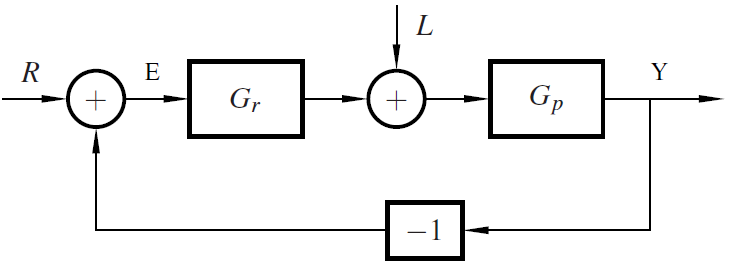
\includegraphics[width=1.0\textwidth]{res/eldiagram.png}
   
\end{center}
\vfill

\newpage
\vfill
\subsection{Bella Scala}
\textit{Mel: Bella Notte}\\
\textit{Inspektorsgyckel Skiphtesgasquen 2023}\\
\index[alfa]{Bella Scala}
\index[anfa]{Åh detta språk, detta ljuvliga språk...}
\begin{parse lines}[\noindent]{#1\\}

Åh detta språk, detta ljuvliga språk,
som vi kallar bella Scala!

Se vilken syn alla uttryck i skyn,
detta ljuva bella Scala!

Fjärran från det du älskar blir koden ödsligt tom,
men i dess närhet sluts du in i dess trolska rikedom.

Åh, åh detta språk, det är ungdomens språk,
som vi kallar bella Scala!
\end{parse lines}
% \null

\newpage
\thispagestyle{empty}
\null
\vfill
\begin{center}
   
   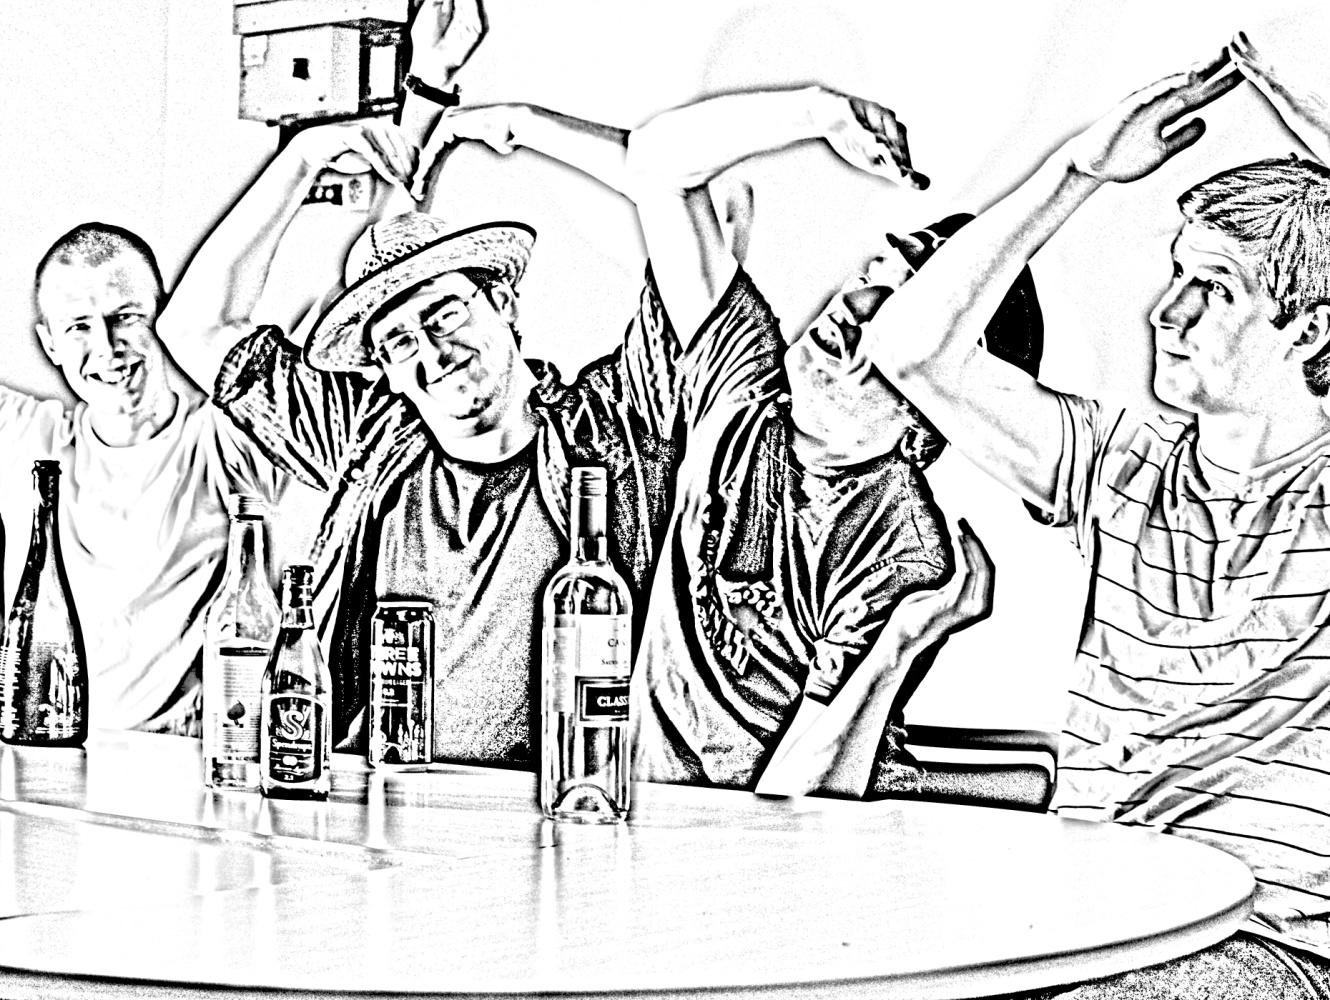
\includegraphics[width=1.0\textwidth]{res/sallskapsvisor.jpg}
   \section{Sällskapsvisor}
\end{center}
\vfill
\newpage



\subsection{Bussången}
\textit{Mel: Jag är en astronaut}\\
\index[alfa]{Bussången}
\index[anfa]{Förr när man skulle bort...}
\begin{parse lines}[\noindent]{#1\\}

Förr när man skulle bort 
lång väg såväl som kort 
fick man ta cykeln eller gå 
nu är det inte så

Fööör...
Nu kan vi åka buss 
förarn bestämmer kurs 
Fönstren är många, ratten rund
här i vår buss från Lund

Nu ska vi leka bin 
här i vår busskabin 
Buzz, buzz, buzz, buzz, buzz, buzz, buzz, buzz 
buzz, buzz, buzz, åka buss!

\end{parse lines}
\vfill
\noindent\textit{Sjungs på varje bussresa.}


\newpage
\subsection{Skolan svämmar över alla breddar}
\textit{Mel: Längtan till landet}\\
\index[alfa]{Skolan svämmar över alla breddar}
\index[anfa]{Skolan svämmar över alla breddar"!}
\begin{parse lines}[\noindent]{#1\\}

Skolan svämmar över alla breddar!
Nu har nollan åter kommit hit.
Nollan vilsen, osäker och rädd är,
ty en nolla vet ju ej ett dugg.

Irra från sektionen till KF-sigma,
famnen full av böcker; vart skall vi nu?
Festa hela natten, sen ska man pigg va;
Föreläsning börjar klockan sju!

Föreläsarn mumlar längst fram i salen,
integraler virvlar; matte är kul!
Varva fest med studier, sen kommer kvalen!
Åtta tentor, sen så är det jul!
\end{parse lines}


\subsection{Skandal}
\textit{Mel: Amazing grace}\\
\index[alfa]{Skandal}
\index[anfa]{Skandal, skandal, skandal, skandal...}
\begin{parse lines}[\noindent]{#1\\}

Skandal, skandal, skandal, skandal. 
Skandal, skandal, skandal. 
Skandal, skandal, skandal, skandal. 
Skandal, skandal, skandal.
\end{parse lines}


\subsection{Grå häst}
\textit{Mel: Go west}\\
\index[alfa]{Grå häst}
\index[anfa]{Grå häst...}
\begin{parse lines}[\noindent]{#1\\}

Grå häst
Jag har skaffat en
Grå häst
Den är född av en 
Grå häst
Den har fyra ben
Grå häst, nu så har den blivit en

Grå väst
Jag har gjort mig en
Grå väst
Den är mjuk och len
Grå väst
Den har fyra ben
Grå väst, efter tvätten blev den en

Grå rest
Den ser ut som en
Grå rest
Ganska homogen
Grå rest
Nu jag hör siren
Grå rest, myndigheten tog mig sen



Arrest
Jag är helt allen
Arrest
Nu är jag blott en
Grå rest
För de hitta en
Grå väst, Ja, jag hade stulit en

Grå häst...
\end{parse lines}

\subsection{Studiemedelsrondo}
\textit{Mel: Lossa sand}\\
\index[alfa]{Studiemedelsrondo}
\index[anfa]{Vi dricker punsch till lunch...}
\begin{parse lines}[\noindent]{#1\\}

Vi dricker punsch till lunch
när vi har fått avin.
Vi lunchar hela dagen
tills kassan gått i sin.
\end{parse lines}

\vfill
\subsection{Teknologvisa}
\textit{Mel: I’m a lumberjack}\\
\index[alfa]{Teknologvisa}
\index[anfa]{Jag är teknolog och helt OK...}

\noindent\textbf{Jag är teknolog och helt OK\\
Jag jobbar hårt och jag roar mig}\\\\
\noindent Han är teknolog och helt OK\\
Han jobbar hårt och han roar sig\\\\
\noindent\textbf{Teknik är ball\\
Jag kan Pascal\\
Till Lophtet vill jag gå\\
Där träffas alla vänner\\
som är från LTH}\\\\
\noindent Teknik är ball\\
Han kan Pascal\\
Till Lophtet vill han gå\\
Där träffas alla vänner\\
som är från LTH\\\\
\noindent För han är teknolog och helt OK\\
Han jobbar hårt och han roar sig\\\\
\noindent\textbf{Min mattebok \\
den gör mig klok\\
Jag läser kärnfysik\\
Jag går på föreläsning\\
och älskar juridik}\\\\
\noindent Hans mattebok\\
den gör han klok\\
Han läser kärnfysik\\
Han går på föreläsning\\
och älskar juridik???\\\\
\noindent Men han är teknolog och helt OK\\
Han jobbar hårt och han roar sig\\\\
\noindent\textbf{Som ekonom jag blir fantom\\
Konkurser gör mig säll\\
Till flickor blankt jag nekar\\
Jag älskar en tabell}\\\\
\noindent Som ekonom han blir fantom???\\
konkurser...\\
Nää, BUU!!\\\\
\noindent Men han är teknolog och helt OK\\
Han jobbar hårt och han roar sig\\

\noindent\textit{Fetstilt sjunges av försångare.}


\newpage
\subsection{Vi klarar oss nog ändå}
\textit{Mel: Vi klarar oss nog ändå}\\
\index[alfa]{Vi klarar oss nog ändå}
\index[anfa]{Jag vill sjunga en visa i klaraste dur...}
\begin{parse lines}[\noindent]{#1\\}

Jag vill sjunga en visa i klaraste dur,
ty den handlar om Skåne å slätter å djur.
Kan hända den retar en del,
men i så fall e det deras eget fel.
Det har talats så mycket om dynga och lort,
men betänk vilken oerhörd nytta den gjort.
Så låt dom bara gå på,
vi klarar oss nog ändå.
Ja, låt dom bara gå på,
vi klarar oss nog ändå.

Kanske språket vi talar ej klingar så väl,
men de e å förbliver en del av vår själ.
Kan hända det retar en del,
men i så fall e det deras eget fel.
Uti självaste riksdan på skånska di slåss,
för de flesta utav dom har kommit från oss.
Så låt dom ...

Hela landet får njuta av vår akvavid,
sockerbedan har lärt dom att dricka på bid.
Kan hända det retar en del,
men i så fall e det deras eget fel.
Våran sandstrand den e både bländvit å fin,
åsså har vi ju vår lilla vida kanin.
Så låt dom ..
\end{parse lines}

\vspace{-0.8cm}
\subsection{Regattasången}
\textit{Mel: Rövarna från Kamomilla stad}\\
\index[alfa]{Regattasången}
\index[anfa]{Regattaslag på LTH...}
\begin{parse lines}[\noindent]{#1\\}

Regattaslag på LTH
På sjön Sjøn ska vi härja
Förstöra allt vi kommer åt
Å dörren ska vi bärga

Båtarna körs ned på ramp
Sektionerna gör upp i kamp

Elektro Kemi Eko ING och Fysik
Data V A Maskin också I-sektion
\end{parse lines}

\vfill
\subsection{Morbid busslåt}
\textit{Mel: Båtlåt}\\
\index[alfa]{Morbid busslåt}
\index[anfa]{Det var en buss som sa till en annan...}
\begin{parse lines}[\noindent]{#1\\}

Det var en buss som sa till en annan:
- Vad du var stilig, din lack är alldeles för grann.
Vi prejas lite grann, och repar ner varann.
Som bara bussar kan.
Badda bam bam bam bam
Badda bam bam bam

Andra bussen sa: - Klart att jag vill va
med och krocka. Krossa din stiliga för.
Vi varann förstör. Busschauffören dör.
Av vägen sen vi kör.
Badda bam bam bam bam
Badda bam bam bam

Sedan kan vi slå, en och kanske två
våldsamma volter. Landa nånstans vid en bäck.
Rulla lite däck. Bensintanken är läck.
Och elden är ej släckt.
Badda bam bam bam bam
Badda bam bam BOOM!
\end{parse lines}

\newpage
\thispagestyle{empty}
\null
\vfill
\begin{center}

   
\includegraphics[width=0.8\textwidth]{res/gamlavisor.png}
   \section{Gamla visor}
   
\end{center}
\vfill
\newpage
\textit{Gamla visor är sånger som varit omtyckta och sjungits på sektionen, men som av olika anledningar arkiverats. Sektionen står inte bakom innehållet i visorna och de sjunges på egen risk.}

\subsection{Supa tills vi stupar}
\textit{Mel: The wild rover}\\
\index[alfa]{Supa tills vi stupar}
\index[anfa]{Vi öla på Malmö, till sång och till skrik...}
\begin{parse lines}[\noindent]{#1\\}

Vi öla på Malmö, till sång och till skrik
Då kom det en grabb, han gick juridik
Han kom fram till vårt bord, kalla oss fulla svin
men det skiter vi i för vi går på Maskin

Vi blir kvar och röjer
Kommer aldrig gå hem
Vi ska supa tills vi stupar
För vi går på M.

Vi öla i parken, då kom den en man
Han hade fått sparken, var sliten som fan
Han sa ”Läs inte data. Ni slösar bort ti’n”
men det skiter vi i för vi går på Maskin

Vi blir kvar…

Vi öla på Sparta, som så ofta har hänt
Då kom det en östtysk utbytesstudent
Han sa ”Tjänare grabbar, vill ni ha lite morfin?”
Nej det skiter vi i, TROTS att vi går på Maskin

Vi blir kvar…

Vi vakna på sjukan, hur fan kom vi dit?
Men där kom nån på här finns ju läkarsprit
Men doktorn sa ”Stopp! Det där är till medicin!”
Men det skiter vi i för vi går på Maskin

Vi blir kvar…
\end{parse lines}


\vfill
\subsection{Dunderdrickan}
\textit{Mel: Itsy bitsy}\\
\index[alfa]{Dunderdrickan}
\index[anfa]{Det var en kväll då jag gick ner till krogen...}
\begin{parse lines}[\noindent]{#1\\}

Det var en kväll då jag gick ner till krogen
för att äta å ta mig ett glas.
Första flaskan kom in och jag drog den,
sedan gick hela kvällen i kras.

"Ett, två, tre, vilken dricka var då det?"

Jo, det var en stark och mäktig dunderdricka,
tappa glaset, börja slicka.
En liten bordssup längs smalbenet rann.
En annan mäktig dunderdricka
fort slank ner, jag börja hicka.
En liten bordssup, mitt minne försvann!

Pam pam pam...

Jag är för full för att ta mig ur stolen.
Jag är för full för att känna min arm.
Jag är så full att jag trilla i poolen.
Jag vakna upp i en storbystad barm.

"Ett, två, tre, men hur kunde detta ske?"

Jo, utav en stark och mäktig dunderdricka
till akuten mig de skicka.
Min lilla bordssup gav leverbesvär.
Men doktorn på mig konstigt titta,
hitta bara sockerdricka,
och sa förbannat "Vad fan gör du här?"
\end{parse lines}

\subsection{Efter alkohol}
\textit{Mel: The money song}\\
\textit{Bordsvisa D-sektionen 2011}\\
\index[alfa]{Efter alkohol}
\index[anfa]{Man har klagat på mitt bordsskick efter supen...}
\begin{parse lines}[\noindent]{#1\\}

Man har klagat på mitt bordsskick efter supen,
Man har anklagat mig för att sjunga falskt.
Det sägs att jag blir fumlig-
efter att min syn blir grumlig.
Men jag tar inte åt mig därför att:

Efter alkohol blir alla runt mig snygga.
Efter alkohol villa va min vän.
Ni säger:- ta det varligt
Medan jag ser inget farligt
Jag tror nog jag ska ta mig ännu en.

Efter alkohol så kan jag plötsligt flyga
Efter alkohol så vågar jag ta sats
Plötsligt blir jag modig, stark och obegripligt rolig
och allt blir möjligt genom alkohol-hol-hol

Jag må va full som fan, men du är likadan
genom öl o vin o cider
får jag alltid ragg!
\end{parse lines}

\vspace{-0.8cm}
\subsection{Här på en skola i Lund}
\textit{Mel: Under en filt i Madrid}\\
\index[alfa]{Här på en skola i Lund}
\index[anfa]{Här på en skola i Lund...}
\begin{parse lines}[\noindent]{#1\\}

Här på en skola i Lund
skulle jag studera en stund
skulle plugga och vara så sund
här på skola i Lund

För tänk innan jag kom hit
drack jag ej en droppe sprit
men här super jag som en hund
här på en skola i Lund

Min studiesituation
har upplevt en evolution
dålig är min prestation
men drycken ger motivation

I ett hav av brännvin och öl
guppar jag runt på fel köl
mina ben gör ej som jag vill
men ge mig en rackare till

För fan här finns bara drägg
kom kyss en kille med skägg
här finns inga tjejer att få
men kom ska jag få den att stå

Kanske tycker du att denna sång
bör inkapslas i en kodong
med den sagga du lade däri
men det skiter jag i

Jag skiter i studierna nu
och knullar med lärarens fru
Om varenda tenta jag kör
kan jag supa här tills jag dör

För fan där gnäggar en get
jag faller till taket som smet
det blir till att däcka en stund
här på skola i Lund
\end{parse lines}
\vfill
\subsection{Jag vill gå på Data-InfoCom}
\textit{Mel: Blommig falukorv}\\
\index[alfa]{Jag vill gå på Data-InfoCom}
\index[anfa]{Jag vill gå på Data-Infocom...}
\begin{parse lines}[\noindent]{#1\\}

Jag vill gå på Data-Infocom
Mamma
Bästa här på LTH
och alla era brudar
de dyrkar oss som gudar
Ja vi står över alla er

E - Löder för mycket
F - Pallar ej trycket
M:arna ser ut som apor

Jag vill gå på Data-Infocom
Pappa
Nått annat vill jag inte gå

Jag hatar kemister, de är som Chalmerister
A har knappt nån nollning alls

W - Dom går åt skogen
I - Snobbar på krogen
V:arna de dricker vatten

Jag vill gå på Data-Infocom
DIN MAMMA!!!
\end{parse lines}


\newpage
\thispagestyle{empty}
\null
\vfill
\begin{center}
   
   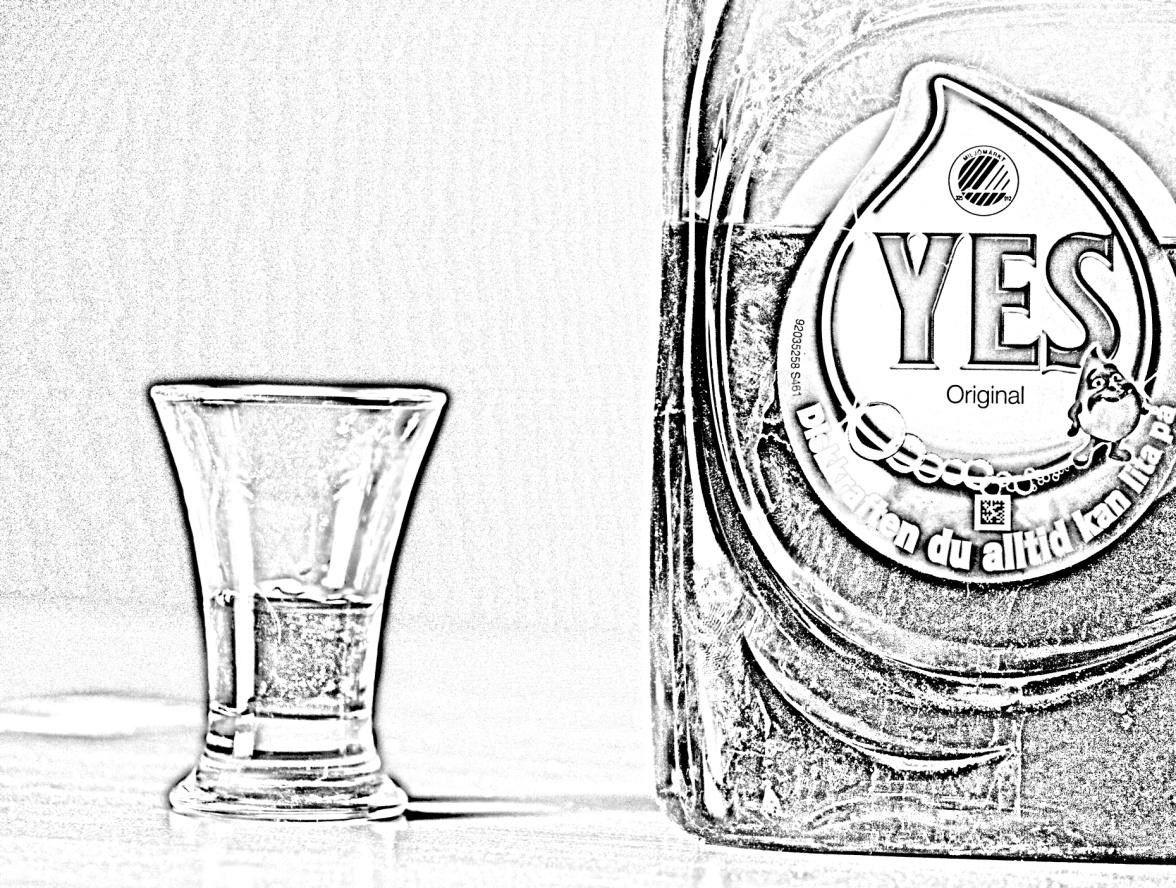
\includegraphics[width=1.0\textwidth]{res/drygavisor.jpg}
   \section{Dryga visor}
\end{center}
\vfill
\newpage

\begin{multicols}{2}
\subsection{Ebbe 1988}
\index[alfa]{Ebbe 1988}
\index[anfa]{Ebbe Ebbe Ebbe...}
\begin{parse lines}[\noindent]{#1\\}
Ebbe Ebbe Ebbe, 
Ebbe, Ebbe.
Ebbe Ebbe Ebbe, 
Ebbe, Ebbe.
Han ville bli polis.

Ebbe Ebbe Ebbe, 
Ebbe,  Ebbe.
Ebbe Ebbe Ebbe, 
Ebbe,  Ebbe.
Han samlade bevis.
\end{parse lines}

\subsection{Abbe 1989}
\index[alfa]{Abbe 1989}
\index[anfa]{Abbe Abbe Abbe...}
\begin{parse lines}[\noindent]{#1\\}
Abbe Abbe Abbe, 
Abbe,  Abbe.
Abbe Abbe Abbe, 
Abbe,  Abbe.
Var nollegeneral.

Abbe Abbe Abbe, 
Abbe,  Abbe.
Abbe Abbe Abbe, 
Abbe,  Abbe.
Han gjorde stor skandal.
\end{parse lines}

\subsection{Nubbe 1990}
\index[alfa]{Nubbe 1990}
\index[anfa]{Nubbe nubbe nubbe...}
\begin{parse lines}[\noindent]{#1\\}
Nubbe nubbe nubbe,
nubbe, nubbe.
Nubbe nubbe nubbe,
nubbe, nubbe.
Den är ljuv och sval.

Nubbe nubbe nubbe,
nubbe, nubbe.
Nubbe nubbe nubbe,
nubbe, nubbe.
Lyckan är total.
\end{parse lines}

\subsection{E:B 1991}
\index[alfa]{E:B 1991}
\index[anfa]{E:B E:B E:B...}
\begin{parse lines}[\noindent]{#1\\}
E:B E:B E:B,
E:B, E:B.
E:B E:B E:B,
E:B, E:B.
Reglerteknik på gång.

E:B E:B E:B,
E:B, E:B. E:B E:B E:B,
E:B, E:B.
Men salen var för trång
\end{parse lines}

\subsection{3-D 1992}
\index[alfa]{3-D 1992}
\index[anfa]{3-D 3-D 3-D...}
\begin{parse lines}[\noindent]{#1\\}
3-D 3-D 3-D
3-D, 3-D.
3-D 3-D 3-D
3-D, 3-D.
En extra dimension.

3-D 3-D 3-D
3-D, 3-D.
3-D 3-D 3-D
3-D, 3-D.
I vår television.
\end{parse lines}

\subsection{VG 1993}
\index[alfa]{VG 1993}
\index[anfa]{VG VG VG...}
\begin{parse lines}[\noindent]{#1\\}
VG VG VG
VG, VG.
VG VG VG
VG, VG.
Nu drar vi ut ett gäng.

VG VG VG
VG, VG.
VG VG VG
VG, VG.
En riktig nöjessväng.
\end{parse lines}

\subsection{BB 1994}
\index[alfa]{BB 1994}
\index[anfa]{BB BB BB...}
\begin{parse lines}[\noindent]{#1\\}
BB BB BB
BB, BB.
BB BB BB
BB, BB.
Sugklocka och tång.

BB BB BB
BB, BB.
BB BB BB
BB, BB.
Vi föddes på en gång!
\end{parse lines}

\subsection{VM 1995}
\index[alfa]{VM 1995}
\index[anfa]{VM SM AM...}
\begin{parse lines}[\noindent]{#1\\}
VM SM AM
EM, NM.
KM IM OM
FM, OS.
Medaljer tusenfalt!

VM SM AM
EM, NM.
KM IM OM
FM, OS.
Norge vinner allt!
\end{parse lines}

\begin{flushleft}
\subsection{Soap Addict 1996}
\index[alfa]{Soap Addict 1996}
\index[anfa]{Dallas, Falcon Crest och...}
\begin{parse lines}[\noindent]{#1\\}
Dallas, Falcon Crest och
Rederiet,
Bevvan, Skilda Världar,
det är givet.
Min fjärrkontroll går varm.
\end{parse lines}
\end{flushleft}
\begin{parse lines}[\noindent]{#1\\}
Varuhuset, Melrose
och Tre Kronor.
Grannar, Dynastin och,
Hem till gården.
Jag får tennisarm!
\end{parse lines}


\subsection{Björne 1997}
\index[alfa]{Björne 1997}
\index[anfa]{Björne Björne Björne...}
\begin{parse lines}[\noindent]{#1\\}
Björne Björne Björne
Björne, Björne.
Björne Björne Björne
Björne, Björne.
Vi ser hans magasin.

Björne Björne Björne
Björne, Björne.
Björne Björne Björne
Björne, Björne.
Fluffig, fet och fin!
\end{parse lines}

\subsection{Skvaller 1998}
\index[alfa]{Skvaller 1998}
\index[anfa]{Skvaller skvaller skvaller...}
\begin{parse lines}[\noindent]{#1\\}
Skvaller skvaller skvaller
skvaller, skvaller.
Skvaller skvaller skvaller
skvaller, skvaller.
Clinton var på glid.

Skvaller skvaller skvaller
skvaller, skvaller.
Skvaller skvaller skvaller
skvaller, skvaller.
Kungen är gravid!
\end{parse lines}


\subsection{B1 \& B2 1999}
\index[alfa]{B1 \& B2 1999}
\index[anfa]{B1 B1 B1...}
\begin{parse lines}[\noindent]{#1\\}
B1 B1 B1,
B1, B1.
B1 B1 B1,
B1, B1.
Vi står här och ler.

B2 B2 B2,
B2, B2.
B2 B2 B2,
B2, B2.
Vi ska skalas ner!
\end{parse lines}

\subsection{Kalle 2000}
\index[alfa]{Kalle 2000}
\index[anfa]{Kalle Kalle Kalle...}
\begin{parse lines}[\noindent]{#1\\}
Kalle Kalle Kalle,
Kalle, Kalle.
Kalle Kalle Kalle,
Kalle, Kalle.
Går på om en minut.

Kalle Kalle Kalle,
Kalle, Kalle.
Kalle Kalle Kalle,
Kalle, Kalle.
Det som vi sett förut!
\end{parse lines}

\vspace{-0.7cm}
\subsection{Ebbe 2001}
\index[alfa]{Ebbe 2001}
\index[anfa]{Killar killar killar...}
\begin{parse lines}[\noindent]{#1\\}
Killar killar killar
killar, killar.
Killar killar killar
killar, killar.
Killarna ska ut.

Tjejer tjejer tjejer,
tjejer, tjejer.
Tjejer tjejer tjejer,
tjejer, tjejer.
Tjejerna ska in.
\end{parse lines}
\vspace{-0.5cm}
\begin{flushleft}
\textit{2002 var Sångarstriden inställd. 2003 inkluderades ingen Ebbe-visa.}
\end{flushleft}
\subsection{Äggda 2004}
\index[alfa]{Äggda 2004}
\index[anfa]{Äggda Äggda Äggda...}
\begin{parse lines}[\noindent]{#1\\}
Äggda Äggda Äggda
Äggda, Äggda.
Äggda Äggda Äggda
Äggda, Äggda.
CF, SIF – Nej, Tack!

Äggda Äggda Äggda
Äggda, Äggda.
Äggda Äggda Äggda
Äggda, Äggda.
Äggen har sitt fack.
\end{parse lines}

\subsection{Sopor 2005}
\index[alfa]{Sopor 2005}
\index[anfa]{Sopor Sopor Sopor...}
\begin{parse lines}[\noindent]{#1\\}
Sopor Sopor Sopor,
Sopor, Sopor.
Sopor Sopor Sopor,
Sopor, Sopor.
Återvinns så lätt.

Sopor Sopor Sopor,
Sopor, Sopor.
Sopor Sopor Sopor,
Sopor, Sopor.
Skräpmat gör mig mätt!
\end{parse lines}

\subsection{Sjön Sjøn 2006}
\index[alfa]{Sjön Sjøn 2006}
\index[anfa]{Sjön Sjøn Sjön Sjøn Sjön Sjøn...}
\begin{parse lines}[\noindent]{#1\\}
Sjön Sjøn sjön Sjøn sjön Sjøn,
sjön Sjøn, sjön Sjøn.
Sjön Sjøn sjön Sjøn sjön Sjøn
sjön Sjøn, sjön Sjøn.
Vattnet som han drack.

Sjön Sjøn sjön Sjøn sjön Sjøn
sjön Sjøn, sjön Sjøn.
Sjön Sjøn sjön Sjøn sjön Sjøn
sjön Sjøn, sjön Sjøn.
Spydde ner en frack.
\end{parse lines}
\begin{flushleft}
\noindent \textit{Sångarstriden 2006 sköts fram till våren 2007. Sedermera sköts även Sångarstriden 2007 fram ett halvår. Data fick då dra sig ur på grund av krock med andra aktiviteter. Materialet sparades dock och användes 2008 istället.}
\end{flushleft}


\subsection{HB 2008}
\index[alfa]{HB 2008}
\index[anfa]{HB HB HB...}
\begin{parse lines}[\noindent]{#1\\}
HB HB HB,
HB, HB.
HB HB HB,
HB, HB.
När kärringen är svår.

HB HB HB,
HB, HB.
HB HB HB,
HB, HB.
Då tar jag mig en tår.
\end{parse lines}

\subsection{Clownens visa 2009}
\index[alfa]{Clownens visa 2009}
\index[anfa]{Ett å två å tre å...}
\begin{parse lines}[\noindent]{#1\\}
Ett å två å tre å,
fyra, fem, sex.
Sju å åtta, nio, 
elva, tretton.
Ett mattegeni

1 + 2 är 4,
3 + 5 är ...
7 + 2 är 11,
18, 33!
Jag går ekonomi!
\end{parse lines}

\subsection{IP 2010}
\index[alfa]{IP 2010}
\index[anfa]{IP IP IP...}
\begin{parse lines}[\noindent]{#1\\}
IP IP IP, 
IP, IP.
IP IP IP,
IP, IP.
Mitt favvoprotokoll

IP IP IP, 
IP, IP.
IP IP IP,
IP, IP.
På adressen har jag koll
\end{parse lines}

\subsection{Tenta 2011}
\index[alfa]{Tenta 2011}
\index[anfa]{Tenta tenta tenta...}
\begin{parse lines}[\noindent]{#1\\}
Tenta tenta tenta, 
tenta, tenta.
Tenta tenta tenta, 
tenta, tenta.
Utan ett annex

Tenta tenta tenta, 
tenta, tenta.
Tenta tenta tenta, 
tenta, tenta.
Schemat blir komplex
\end{parse lines}


\subsection{Plugga 2012}
\index[alfa]{Plugga 2012}
\index[anfa]{Plugga plugga plugga...}
\begin{parse lines}[\noindent]{#1\\}
Plugga plugga plugga
plugga plugga
plugga plugga plugga
plugga plugga
36 veckor per år

Plugga plugga plugga
plugga plugga
plugga plugga plugga
plugga plugga
snart 40 om 'nåt år
\end{parse lines}
\vspace{-0.4cm}
\subsection{Ebbe 2013}
\index[alfa]{Ebbe 2013}
\index[anfa]{Jag har sett dig genom dina fönster...}
\begin{parse lines}[\noindent]{#1\\}
Jag har sett dig genom dina fönster
Jag kan se dina vanor, dina mönster
Vill du bli min fru?

Gå inte med honom
han är creepy
kom med mig istället
ner till Afrika
och rädda alla barn
\end{parse lines}
\vspace{-0.3cm}

\begin{flushleft}
\noindent\textit{Datatekniksektionen deltog inte i Sångarstriden 2014.}
\end{flushleft}

\subsection{Ebbe 2015}
\index[alfa]{Ebbe 2015}
\index[anfa]{Hen har sett dig genom...}
\begin{parse lines}[\noindent]{#1\\}
Hen har sett dig genom
tinder-appen
kom igen nu svara
öppna snappen
du gör vad som helst

Hen är ganska pryd och
riktigt kristen
ondheten hos dig du,
den e briiiisten
gå nu och bli frälst
\end{parse lines}
\vspace{-0.4cm}
\subsection{Sallad 2016}
\index[alfa]{Sallad 2016}
\index[anfa]{Sallad, sallad, sallad...}
\begin{parse lines}[\noindent]{#1\\}
Sallad, sallad, sallad
Sallad, sallad
Sallad, Salas, sallad
sallad, saaaallad
makten är för stor

Sallad, sallad, sallad
Sallad, sallad
Sallad, sallad, sallad
sallad, saaallad
sallad, sallad, sall.
\end{parse lines}

\subsection{Ketchup 2017}
\index[alfa]{Ketchup 2017}
\index[anfa]{Tar du denna tomat...}
\begin{parse lines}[\noindent]{#1\\}
Tar du denna tomat
Som din make
Ser till att älska honom
Hela livet ut
Det gör jag såklart

Tar du denna tomat
Som din maka
Ser till att älska henne
Hela livet ut
Verkligen absolut
\end{parse lines}
\vspace{-0.8cm}
\subsection{Ladok 2018}
\index[alfa]{Ladok 2018}
\index[anfa]{Välkomna till tentan här...}
\begin{parse lines}[\noindent]{#1\\}
Välkomna till tentan
här i kårgasque
Häng av jackan här o 
stäng av telefonen.
Inga hjälpmedel.
Jag kan inte hitta 
dig på listan. 
Har du inte anmält 
dig i laaaadok?
Ladok var ju stängt
Står du ej på listan, 
får jag be dig
Lämna tentasalen, 
ögonblickligen
Ge dig genast av!
\end{parse lines}
\end{multicols}








\subsection{Min gode vän Joel}
\textit{Mel: Trampa på gasen}\\
\index[alfa]{Min gode vän Joel}
\index[anfa]{Min gode vän Joel...}
\begin{parse lines}[\noindent]{#1\\}

Min gode vän Joel,
han är en glad kamrat,
Han har äpplen fram och en kulvert bak.

Min gode vän Joel,
han ser rätt lustig ut.
Man kan kalla honom Knut,
om man vill,
och det vill man.
\end{parse lines}


\subsection{Min gode vän Jor-El}
\textit{Mel: Trampa på gasen}\\
\index[alfa]{Min gode vän Jor-El}
\index[anfa]{Min gode vän Jor-El...}
\begin{parse lines}[\noindent]{#1\\}

Min gode vän Jor-El, 
är far till Superman.
Super man som han blir man full som fan!
Min gode vän Jor-El, 
han dricker supersprit,
men tål inte kryptonit!
Kastar upp
i raketen!
\end{parse lines}

\subsection{Bortom IT-samhället}
\textit{Mel: Trampa på gasen}\\
\index[alfa]{Bortom IT-samhället}
\index[anfa]{Usama bin Laden...}
\begin{parse lines}[\noindent]{#1\\}

Usama bin Laden
har ingen SMS,
ingen ICQ eller mailadress.
Usama bin Laden
tycks ha gått upp i rök,
man kan inte klicka 'Sök'
om man vill,
och det vill Bush (fortfarande)!
\end{parse lines}


\subsection{Den kuggade tentans visa}
\textit{Mel: Trampa på gasen}\\
\index[alfa]{Den kuggade tentans visa}
\index[anfa]{Jag kuggade tentan...}
\begin{parse lines}[\noindent]{#1\\}

Jag kuggade tentan
men det gör inte nått
för jag hade ändå inga pengar fått
för om man blir ratad
av hela CSN
får man ofta ringa hem
för att få lite pengar
\end{parse lines}

\vfill
\subsection{Jag pluggar på LU}
\textit{Mel: Trampa på gasen}\\
\index[alfa]{Jag pluggar på LU}
\index[anfa]{Jag pluggar på LU...}
\begin{parse lines}[\noindent]{#1\\}

Jag pluggar på LU,
och läser gratispoäng.
När ni gör er labb,
ligger jag i säng.

Jag pluggar på LU,
tar inga hårda tag.
Men ändå får jag bidrag,
från CSN, ja det får jag!
\end{parse lines}
\vfill
\subsection{Kalmarevisan}
\textit{Mel: Kalmare stad}\\
\index[alfa]{Kalmarevisan}
\index[anfa]{Uti Kalmare stad...}
\begin{parse lines}[\noindent]{#1\\}

Uti Kalmare stad,
ja där finns det ingen kvast
förrän lördagen.
Hej dick! Hej dack!
Jag slog i 
och vi drack.
Hej dickom dickom dack,
hej dickom dickom dack.
För uti Kalmare stad,
ja där finns det ingen kvast
förrän lördagen.

$\vert\vert$: När som bonden kommer hem
kommer bondekvinnan ut :$\vert\vert$
Är så stor i sin trut.
Hej ...

$\vert\vert$: Var är pengarna du fått?
Jo, dem har jag supit opp :$\vert\vert$
uppå Kalmare slott.
Hej ...

$\vert\vert$: Jag ska klaga dig an
för vår Kronbefallningsman :$\vert\vert$
Och du ska få skam.
Hej ...

$\vert\vert$: Kronbefallningsmannen vår
satt på krogen igår :$\vert\vert$
och var full som ett får.
Hej ...
\end{parse lines}


\vfill
\subsection{Måsen}
\textit{Mel: När månen vandrar}\\
\index[alfa]{Måsen}
\index[anfa]{Det satt en mås på en klyvarbom...}
\begin{parse lines}[\noindent]{#1\\}

Det satt en mås på en klyvarbom,
och tom i krävan var kräket.
Och tungan lådde i skepparns gom
där han satt uti bleket.
Jag vill ha sill hördes måsen rope,
och skepparn svarte: Jag vill ha OP,
om blott jag får, om blott jag får.

Nu lyfter måsen från klyvarbom
och vinden spelar i tågen.
OP:n svalkat har skepparns gom.
Jag önskar blott att jag såg 'en.
Så nöjd och lycklig, den arme saten,
han sätter storsegel den krabaten.
Till sjöss han far, och halvan tar.

Den mås som satt på en klyvarbom,
den är nu död och begraven,
Och skepparn som drack en flaska rom,
han har nu drunknat i haven.
Så kan det gå om man fått för mycke,
om man för brännvin har fattat tycke.
Vi som har kvar, vi resten tar. 
\end{parse lines}


\subsection{Anna: en disslåt}
\textit{Mel: När månen vandrar}\\
\index[alfa]{Anna: en disslåt}
\index[anfa]{Min kompis Anna, hon är en bot...}
\begin{parse lines}[\noindent]{#1\\}

Min kompis Anna, hon är en bot
Hon rensar upp i kanalen
Och varje gång jag hör hennes låt
Så får jag ont i analen.
Jag är så trött på den jävla låten
Kan någon vänlig själ banna boten?
Jag vete fan
Jag fick en ban
\end{parse lines}


\subsection{Att tenta matstat}
\textit{Mel: När månen vandrar}\\
\index[alfa]{Att tenta matstat}
\index[anfa]{Jag tänker tenta matstat nån gång...}
\begin{parse lines}[\noindent]{#1\\}

Jag tänker tenta matstat nån gång
jag tänker ta dom poängen
förra tentan blev inte lång
jag borde stannat i sängen
Den jävla kursen, den gör mig galen
Jag tror jag skyller, på karnevalen
och tar den sen i framtiden!
\end{parse lines}

\vfill
\subsection{Fotboll på Fäladen}
\textit{Mel: När månen vandrar}\\
\index[alfa]{Fotboll på Fäladen}
\index[anfa]{Det hände långt ut på Fäladen...}
\begin{parse lines}[\noindent]{#1\\}

Det hände långt ut på Fäladen,
jag skulle utöva fotboll.
Tog i för lite och tränaren,
han blev förtvivlad vid tolv-noll.

Jag våga inget, kapitulera,
men tränarn fortsatte propagera:
- Var ingen mes, det finns protes!
\end{parse lines}


\subsection{Groggen}
\textit{Mel: När månen vandrar}\\
\index[alfa]{Groggen}
\index[anfa]{Jag har nu blandat en helt ny grogg...}
\begin{parse lines}[\noindent]{#1\\}

Jag har nu blandat en helt ny grogg,
som gör mig full som en tunna.
Receptet skriver jag på min blogg,
så att andra ska kunna.
En Rom-o-cola, fast utan Cola
och mera rom, för vi ska ej snåla.
En god idé, den blir succé 
\end{parse lines}

\vfill
\subsection{JAS:en}
\textit{Mel: När månen vandrar}\\
\index[alfa]{JAS:en}
\index[anfa]{Där flög en JAS över Västerbron...}
\begin{parse lines}[\noindent]{#1\\}

Där flög en JAS över Västerbron
Men styrsystemet var trasigt
Piloten sköt ut sig med kanon
För planet svängde så knasigt
"Jag vill ju uppåt, jag vill ju mer"
Men planet svarte: "Jag vill ju ner
Mot alla hjon, på Västerbron"
\end{parse lines}


\subsection{Kompistipset}
\textit{Mel: När månen vandrar}\\
\index[alfa]{Kompistipset}
\index[anfa]{Min kompis Bosse, en bigamist...}
\begin{parse lines}[\noindent]{#1\\}

Min kompis Bosse, en bigamist,
tar alltid två öl i baren.
Han säger "Allting kan verka trist,
ifall man blott bara tar en,
Nej, ta och skaffa dig en till fru å
be alltid bartendern om en duo.
Så skål min vän, och skål igen!"
\end{parse lines}

\vfill
\subsection{Mesen}
\textit{Mel: När månen vandrar}\\
\index[alfa]{Mesen}
\index[anfa]{Det satt en mes i en klyvarmast...}
\begin{parse lines}[\noindent]{#1\\}

Det satt en mes i en klyvarmast
där sågs han ragla och svaja
För trots att frön var hans enda last
var han full som en kaja
"Vad har du gjort!" hördes skepparn stöna
och mesen svarte "Jag rökte fröna
i egen holk, i egen holk."
\end{parse lines}


\subsection{Moosen}
\textit{Mel: När månen vandrar}\\
\index[alfa]{Moosen}
\index[anfa]{Det satt en älg i en klyvartopp...}
\begin{parse lines}[\noindent]{#1\\}

Det satt en älg i en klyvartopp
Förklädd i älgjaktens månad
Han var befjädrad till horn och kropp
Och skepparn blev smått förvånad
"Jag är en mås, goa skepparn" ljög den 
förklädda älgen, därefter flög den
Mjukt föll han sen
På skepparen
\end{parse lines}

\vfill
\subsection{Musen}
\textit{Mel: När månen vandrar}\\
\index[alfa]{Musen}
\index[anfa]{Det satt en mus i en hushållsost...}
\begin{parse lines}[\noindent]{#1\\}

Det satt en mus i en hushållsost
och åt och åt utan måtta
tills osten blivit en mushåls-ost
och han en klotformad råtta
"Så bra", sa musen, "att va en fettboll,
nu kan jag rulla med hast åt rätt håll:
Ostindien! Ostindien!"
\end{parse lines}

\subsection{När månen vandrar}
\textit{Mel: När månen vandrar}\\
\index[alfa]{När månen vandrar}
\index[anfa]{När månen vandrar sin tysta ban...}
\begin{parse lines}[\noindent]{#1\\}

När månen vandrar sin tysta ban
Och tittar in genom rutan
Då tänker jag, att på ljusan dan,
då kan jag klara mig utan.
Då kan jag klara mig utan måne,
men utan Renat och utan Skåne?
Det vete fan, det vete fan.
\end{parse lines}

\newpage
\subsection{Röda havet}
\textit{Mel: Skrattvisa ur Orfeus i underjorden}\\
\index[alfa]{Röda havet}
\index[anfa]{Vi gingo ned till Röda Havet...}
\begin{parse lines}[\noindent]{#1\\}

Vi gingo ned till Röda Havet.
Vi lågo i där minst en kvart,
ja minst en kvart.
Men inte blev vi röda av 'et,
men Röda Havet det blev svart.

Men utav akvavit,
människan till kropp och själ
blir oskuldsfull och vit.
Men utav akvavit,
människan till kropp och själ
blir oskuldsfull och vit.
\end{parse lines}


\subsection{Finska viken}
\textit{Mel: Skrattvisa ur Orfeus i underjorden}\\
\index[alfa]{Finska viken}
\index[anfa]{Vi gingo ner till finska viken...}
\begin{parse lines}[\noindent]{#1\\}

Vi gingo ner till finska viken.
Vi lågo i där minst en kvart,
ja minst en kvart.
Men inte blev vi av med skiten,
men finska viken den blev svart.

Men utav akvavit…
\end{parse lines}


\subsection{Stadsparksdammen}
\textit{Mel: Skrattvisa ur Orfeus i underjorden}\\
\index[alfa]{Stadsparksdammen}
\index[anfa]{Vi gingo ner till stadsparksdammen...}
\begin{parse lines}[\noindent]{#1\\}

Vi gingo ner till stadsparksdammen.
Vi lågo i där minst en kvart,
ja minst en kvart.
Men inte blev vi av med skammen,
men stadsparksdammen den blev svart.

Men utav akvavit...
\end{parse lines}


\subsection{Systembolaget}
\textit{Mel: Skrattvisa ur Orfeus i underjorden}\\
\index[alfa]{Systembolaget}
\index[anfa]{Vi gingo ner till Systembolaget...}
\begin{parse lines}[\noindent]{#1\\}

Vi gingo ner till Systembolaget.
Vi stod i kö där minst en kvart,
ja minst en kvart.
Men inte blev vi fulla av det, 
men systembolaget det gick back.

Men utav akvavit...
\end{parse lines}

\newpage
\subsection{Bastubadet}
\textit{Mel: Skrattvisa ur Orfeus i underjorden}\\
\index[alfa]{Bastubadet}
\index[anfa]{Vi gingo bort till bastubadet...}
\begin{parse lines}[\noindent]{#1\\}

Vi gingo bort till bastubadet
vi satt där inne minst en kvart
men satt för nära aggregatet
så stjärten den blev svart

Men utav akvavit...
\end{parse lines}


\subsection{Vi gingo ner till Edekvata}
\textit{Mel: Skrattvisa ur Orfeus i underjorden}\\
\index[alfa]{Vi gingo ner till Edekvata}
\index[anfa]{Vi gingo ned till Edekvata...}
\begin{parse lines}[\noindent]{#1\\}

Vi gingo ned till Edekvata.
Vi olja borden minst en kvart,
ja minst en kvart.
Men manualen den vi rata,
så Edekvata det blev svart.

Men utav akvavit...
\end{parse lines}

\newpage
\subsection{Lablokalen}
\textit{Mel: Skrattvisa ur Orfeus i underjorden}\\
\index[alfa]{Lablokalen}
\index[anfa]{Vi gingo ned till lablokalen...}
\begin{parse lines}[\noindent]{#1\\}

Vi gingo ned till lablokalen.
Vi var där inne minst en kvart,
ja minst en kvart.
Men inte blev vi av med kvalen,
men lablokalen den blev svart.

Men utav akvavit...
\end{parse lines}


\subsection{Lommabukten}
\textit{Mel: Skrattvisa ur Orfeus i underjorden}\\
\index[alfa]{Lommabukten}
\index[anfa]{Vi gingo ner till Lommabukten...}
\begin{parse lines}[\noindent]{#1\\}

Vi gingo ner till Lommabukten.
Vi lågo i där minst en kvart,
ja minst en kvart.
Men inte blev vi av med lukten,
men Lommabukten den blev svart.

Men utav akvavit...
\end{parse lines}

\vfill
\subsection{Karnevalen}
\textit{Mel: Skrattvisa ur Orfeus i underjorden}\\
\index[alfa]{Karnevalen}
\index[anfa]{Vi gingo ner till karnevalen...}
\begin{parse lines}[\noindent]{#1\\}

Vi gingo ner till karnevalen
och stod i kö där minst tre kvart.
Vi ville in i AF-salen
men inte fan kom vi nånvart.

För utav kösystem
blir det bara skit och allmänna problem.
För utav kösystem
blir det bara problem.

Och vi kom fram till kravallstaketet
och stod kvar där minst en kvart.
Men vi var fast i köhelvetet
så inte fan kom vi nånvart.

För utav kösystem…
\end{parse lines}




\newpage
\thispagestyle{empty}
\null
\vfill
\begin{center}
   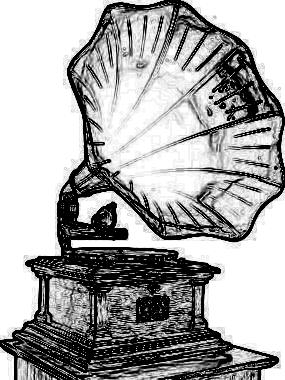
\includegraphics[width=0.8\textwidth, frame]{res/klassiskavisor.jpg}
   \section{Klassiska visor}
\end{center}
\vfill
\newpage



\newpage
\subsection{Du gamla du fria}
\textit{Mel: Du gamla du fria}\\
\index[alfa]{Du gamla du fria}
\index[anfa]{Du gamla, Du fria, Du fjällhöga nord...}
\begin{parse lines}[\noindent]{#1\\}

Du gamla, Du fria, Du fjällhöga nord
Du tysta, Du glädjerika sköna!
Jag hälsar Dig, vänaste land uppå jord,
Din sol, Din himmel, Dina ängder gröna.
Din sol, Din himmel, Dina ängder gröna.

Du tronar på minnen från fornstora dar,
då ärat Ditt namn flög över jorden.
Jag vet att Du är och Du blir vad du var.
Ja, jag vill leva jag vill dö i Norden.
Ja, jag vill leva jag vill dö i Norden.

Jag städs vill dig tjäna mitt älskade land,
din trohet till döden vill jag svära.
Din rätt, skall jag värna, med håg och med hand,
din fana, högt den bragderika bära.
din fana, högt den bragderika bära.

Med Gud skall jag kämpa, för hem och för härd,
för Sverige, den kära fosterjorden.
Jag byter Dig ej, mot allt i en värld
Nej, jag vill leva jag vill dö i Norden.
Nej, jag vill leva jag vill dö i Norden.
\end{parse lines}


\subsection{Nu grönskar det}
\textit{Mel: Nu grönskar det}\\
\index[alfa]{Nu grönskar det}
\index[anfa]{Nu grönskar det i dalens famn...}
\begin{parse lines}[\noindent]{#1\\}

Nu grönskar det i dalens famn,
nu doftar äng och lid.
Kom med, kom med på vandringsfärd
i vårens glada tid!
Var dag är som en gyllne skål,
till brädden fylld med vin.
Så drick, min vän, drick sol och doft,
ty dagen den är din.

Långt bort från stadens gråa hus
vi glatt vår kosa styr,
och följer vägens vita band
mot ljusa äventyr.
Med öppna ögon låt oss se
på livets rikedom
som gror och sjuder överallt
där våren går i blom!
\end{parse lines}
\newpage

\subsection{Always look on the bright side of life}
\textit{Mel: Always look on the bright side of life}
\index[alfa]{Always look on the bright side of life...}
\index[anfa]{}\\
\begin{parse lines}[\noindent]{#1\\}
Ur Monty Pythons “Life of Brian”

Some things in life are bad
They can really make you mad
Other things just make you swear and curse.
When you're chewing on life's gristle
Don't grumble, give a whistle
And this'll help things turn out for the best...

And...always look on the bright side of life...
Always look on the light side of life... 

If  life seems jolly rotten
There's something you've forgotten
And that's to laugh and smile and dance and sing. When you're feeling in the dumps
Don't be silly chumps, ust purse your lips and whistle - that's the thing.

And...always look on the bright side of life...
Always look on the light side of life... 

For life is quite absurd
And death's the final word
You must always face the curtain with a bow.
Forget about your sin - give the audience a grin
Enjoy it - it's your last chance anyhow.

So always look on the bright side of death
Just before you draw your terminal breath 

Life's a piece of shit
When you look at it
Life's a laugh and death's a joke, it's true.
You'll see it's all a show
Keep 'em laughing as you go
Just remember that the last laugh is on you.

And always look on the bright side of life...
Always look on the right side of life...
Always look on the bright side of life...
Always look on the bright side of life...
\end{parse lines}
\textit{(Worse things happen at sea, you know.)}\\
Always look on the bright side of life...\\
\textit{(You know, you come from nothing - you're going back to nothing.\\
What have you lost? Nothing!)}\\
Always look on the right side of life...

\newpage

\subsection{Balladen om herr Fredrik Åkare och den söta fröken Cecilia Lind}
\textit{Mel: Cecilia Lind}\\
\textit{Skriven av Cornelis Vreeswijk}\\
\index[alfa]{Balladen om herr Fredrik Åkare...}
\index[anfa]{Från Öckerö loge hörs dragspel och bas...}
\begin{parse lines}[\noindent]{#1\\}

Från Öckerö loge hörs dragspel och bas
fullmånen lyser som var den av glas
Där dansar Fredrik Åkare kind emot kind
med lilla fröken Cecilia Lind

Hon dansar och blundar så nära intill
Hon följer i dansen precis vart han vill
Han för och hon följer lätt som en vind
Men säg varför rodnar Cecilia Lind?

Säg var det för det Fredrik Åkare sa
"Du doftar så gott och du dansar så bra
Din midja är smal och barmen är trind
Vad du är vacker, Cecilia Lind!"

Men dansen tog slut och vart skulle dom gå?
Dom bodde så nära varandra ändå.
Till slut kom dom fram till Cecilias grind.
"Nu vill jag bli kysst", sa Cecilia Lind

Vet hut Fredrik Åkare, skäms gamla karl
Cecilia Lind är ju bara ett barn
Ren som en blomma, skygg som en hind
"Jag fyller snart sjutton", sa Cecilia Lind

Och stjärnorna vandra och timmarna fly
Och Fredrik är gammal, men månen är ny
Ja, Fredrik är gammal men kärlek är blind
"Kyss mig igen!", sa Cecilia Lind
\end{parse lines}


\subsection{Studentsången}
\textit{Mel: Studentsången}\\
\index[alfa]{Studentsången}
\index[anfa]{Sjungom studentens lyckliga dag...}
\begin{parse lines}[\noindent]{#1\\}

Sjungom studentens lyckliga dag,
låtom oss fröjdas i ungdomens vår!
Än klappar hjärtat med friska slag,
och den ljusnande framtid är vår.
Inga stormar än
i våra sinnen bo,
hoppet är vår vän,
och vi dess löften tro,
när vi knyta förbund i den lund,
där de härliga lagrarna gro!
där de härliga lagrarna gro!
Hurra!
\end{parse lines}

\newpage 

\subsection{Brevet från kolonien}
\textit{Mel: Brevet från kolonien}\\
\textit{Skriven av Cornelis Vreeswijk }\\
\index[alfa]{Brevet från kolonien}
\index[anfa]{Hejsan morsan, hejsan stabben"!}
\begin{parse lines}[\noindent]{#1\\}

Hejsan morsan, hejsan stabben!
Här är brev från älsklingsgrabben.
Vi har kul på kolonien,
vi bor 28 gangstergrabbar i en

Stor barack med massa sängar.
Kan ni skicka mera pengar?
För det vore en god gärning
Jag har spelat bort vartenda dugg på tärning.

Här är roligt vill jag lova
fastän lite svårt att sova
killen som har sängen över mig
Han vaknar inte han när han behöver nej.

Jag har tappat två framtänder
för jag skulle gå på händer
när vi lattjade charader
så när morsan nu får se mig får hon spader.

Ute i skogen finns baciller
men min kompis han har piller
som han köpt utav en ful typ,
och om man äter dom blir man en jättekul typ.

Föreståndaren han har farit
han blir aldrig vad han varit,
för polisen kom och tog hand
om honom förra veckan när vi lekte skogsbrand.

Ute i skogen finns det rådjur,
i baracken finns det smådjur
och min bäste kompis Tage
han har en liten fickkniv inuti sin mage.

Honom ska dom operera,
ja nu vet jag inget mera
kram och kyss och hjärtligt tack sen,
men nu ska vi ut och bränna grannbaracken!
\end{parse lines}
\newpage
\subsection{Incestvisan}
\index[alfa]{Incestvisan}
\index[anfa]{Först träffade jag Marie-Louise...}\textit{Skriven av Cornelis Vreeswijk}\\
\begin{parse lines}[\noindent]{#1\\}
Först träffade jag Marie-Louise 
och jösses vad jag blev kär. 
Vi tänkte väl förlova oss, men min pappa sa tyvärr.
Håll fingrarna ifrån den damen min son 
och sky henne som pest. 
För du och hon har samma far och då blir det incest.

Sen träffade jag Linnea och vi prasslade en tid.
Sen kunde det inte hjälpas att Linnea blev gravid.
När hennes mor fick se min far så stämde hon upp ett tjut. Linnea var min syster och sen fick vi göra slut.

Anita och Carina, Britt-Louise och Siv.
Ja, hundra andra damer fick jag stryka ur mitt liv.
För pappa kände deras mor och sade till direkt.
Den kan du inte gifta dig med för ni är faktiskt släkt.

Förstår du nu medborgare att jag blev ganska sne.
Varenda dam i våran by var jag besläktad med.
Mitt sexualliv krånglade till aska blev min glöd.
Så jag gick till min mamma jag och klagade min nöd.

(Då sa mamma så här:)
Min käre son sa mamma då uti all enkelhet.
Din pappa är en jävla bock som alla människor vet.
Och alla dessa damer är han säkert upphov till.
Men han är inte far till dig så gift dig med vem du vill.
\end{parse lines}
 \vspace{-0.8cm}
\subsection{Drunken sailor}\index[alfa]{Drunken sailor}
\textit{Mel: Drunken sailor}\\
\index[alfa]{Drunken sailor}
\index[anfa]{What shall we do with the drunken sailor...}
\begin{parse lines}[\noindent]{#1\\}

What shall we do with the drunken sailor,
What shall we do with the drunken sailor,
What shall we do with the drunken sailor,
Early in the morning?

Hooray and up she rises, (x3)
Early in the morning!

Put him in the longboat till he's sober, (x3)
Early in the morning!

Hooray and up…

Put 'im in the bilge an' make 'im drink it, (x3)
Early in the morning!

Hooray and up…

Put him in a leaky boat and make him bale it, (x3)
Early in the morning!

Hooray and up…

Shave his belly with a rusty razor, (x3)
Early in the morning!
\end{parse lines}


\subsection{Kungssången}\index[alfa]{Kungssången}
\textit{Mel: Kungssången}\\
\index[alfa]{Kungssången}
\index[anfa]{Ur svenska hjärtans djup en gång...}
\begin{parse lines}[\noindent]{#1\\}

Ur svenska hjärtans djup en gång
en samfälld och en enkel sång,
som går till kungen fram!
Var honom trofast och hans ätt,
gör kronan på hans hjässa lätt,
och all din tro till honom sätt,
du folk av frejdad stam!

O konung, folkets majestät
är även ditt: beskärma det
och värna det från fall!
Stå oss all världens härar mot,
vi blinka ej för deras hot:
vi lägga dem inför din fot -
en kunglig fotapall.

Du himlens Herre, med oss var,
som förr du med oss varit har,
och liva på vår strand
det gamla lynnets art igen
hos sveakungen och hans män.
Och låt din ande vila än
utöver nordanland!
\end{parse lines}


\subsection{Längtan till landet}\index[alfa]{Längtan till landet}
\textit{Mel: Längtan till landet}\\
\index[alfa]{Längtan till landet}
\index[anfa]{Vintern rasat ut bland våra fjällar...}
\begin{parse lines}[\noindent]{#1\\}

Vintern rasat ut bland våra fjällar,
drivans blommor smälta ned och dö.
Himlen ler i vårens ljusa kvällar,
solen kysser liv i skog och sjö.
$\vert\vert$: Snart är sommarn här i purpurvågor,
guldbelagda, azurskiftande
ligga ängarne i dagens lågor,
och i lunden dansa källorne. :$\vert\vert$

Ja, jag kommer! Hälsen, glada vindar,
ut till landet, ut till fåglarne,
att jag älskar dem, till björk och lindar,
sjö och berg, jag vill dem återse,
$\vert\vert$: Se dem än som i min barndoms stunder
följa bäckens dans till klarnad sjö,
trastens sång i furuskogens lunder,
vattenfågelns lek kring fjärd och ö. :$\vert\vert$
\end{parse lines}
\newpage
\null
\newpage
\thispagestyle{empty}
\null
\vfill
\begin{center}
   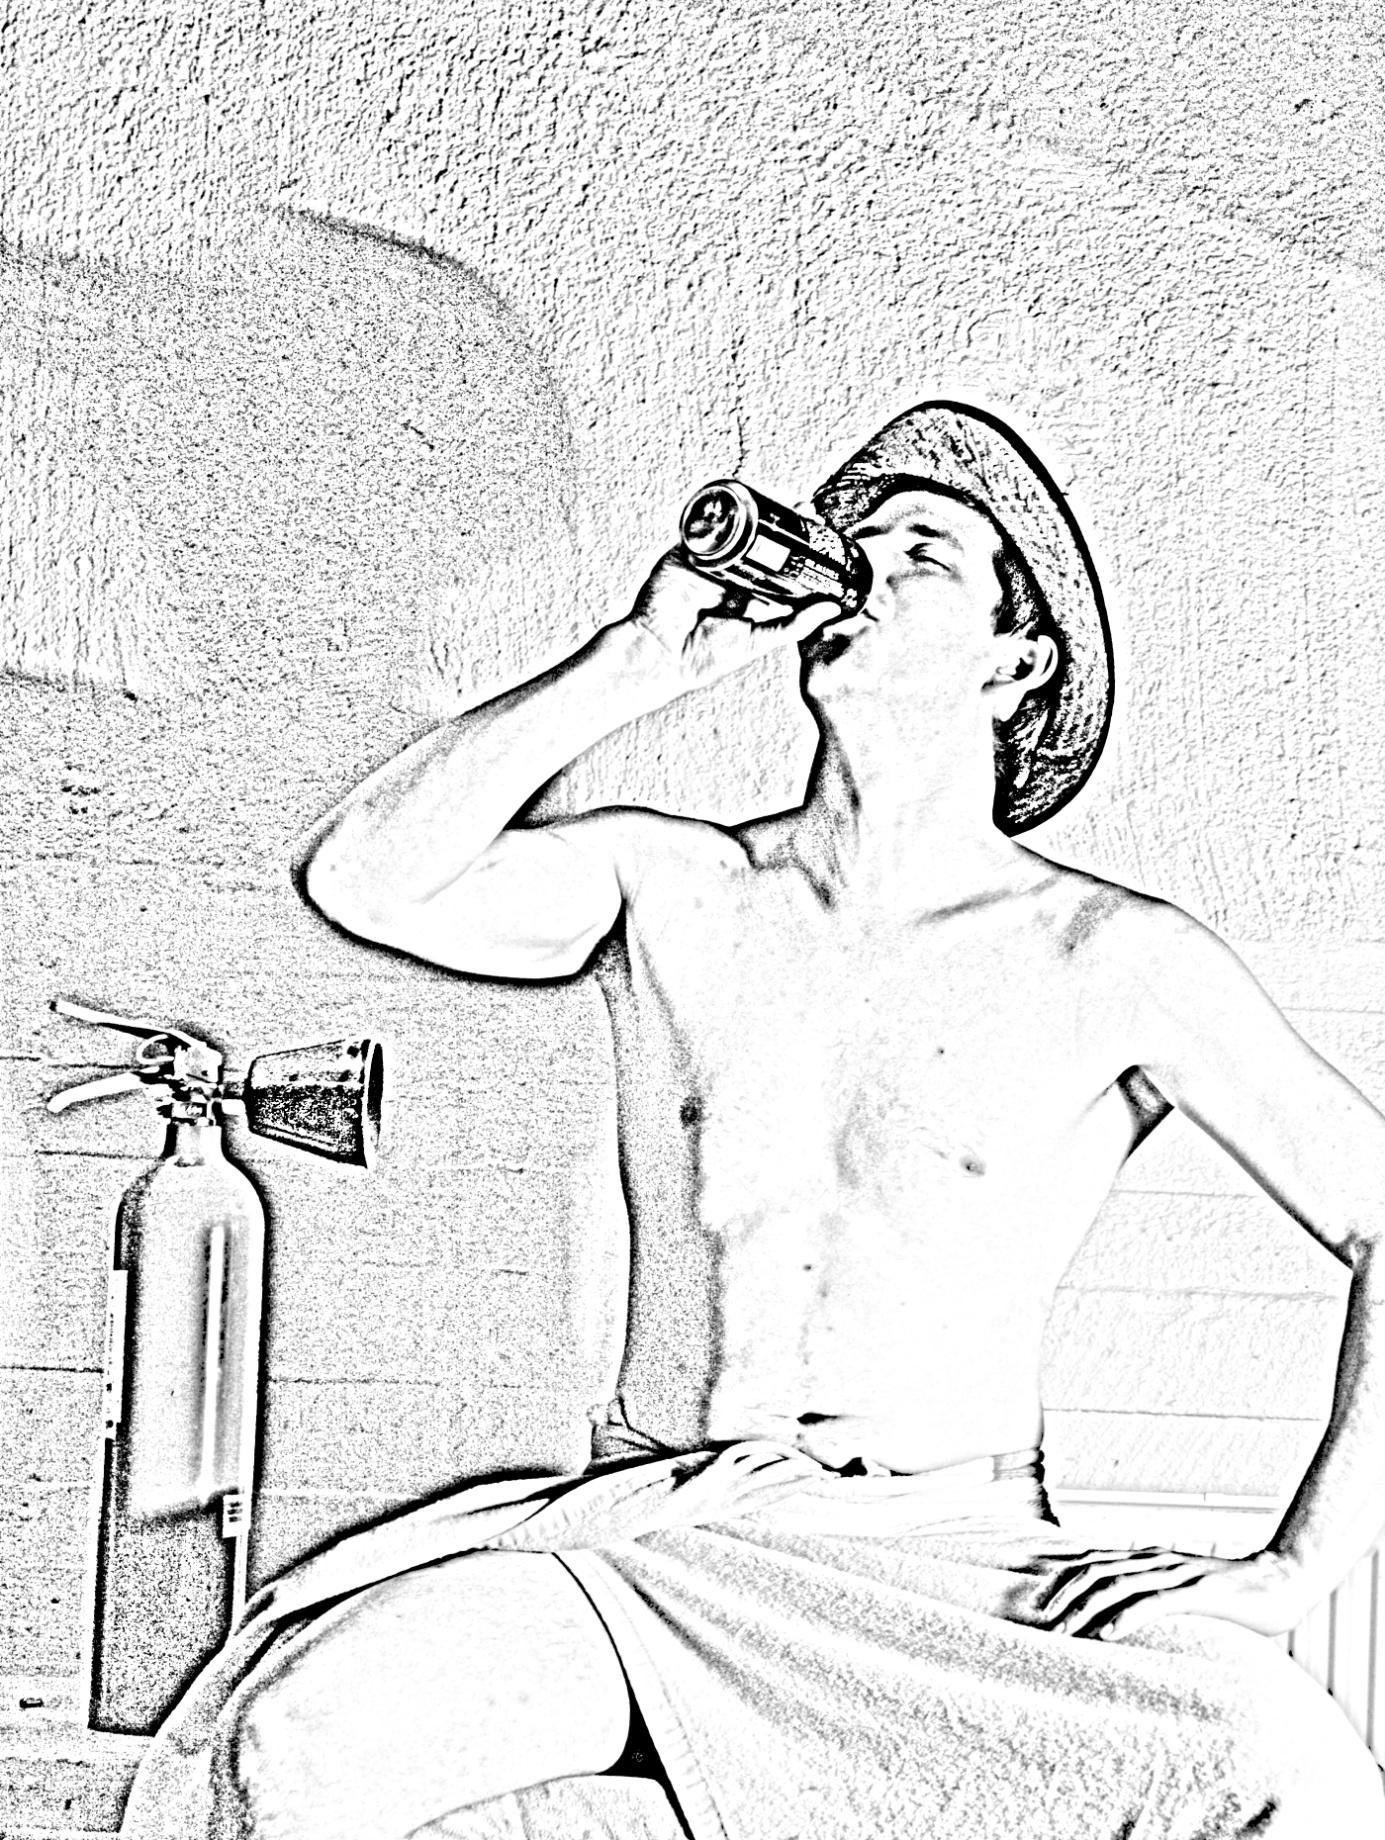
\includegraphics[width=0.8\textwidth, frame]{res/friavisor.jpg}
   \section{Fria visor}
\end{center}
\vfill
\newpage
\noindent\textit{Följande sidor kan användas för att lägga till visor du saknar i denna bok}
\newpage 
\fillInPages{11}


\printindex[alfa]
\printindex[anfa]
\newpage
\thispagestyle{empty}
\subsection{Bortsupen}
\bortsupen[10.5pt]{14}{\textwidth}
\end{document}